% CSML Final Project Paper

\documentclass[11pt,a4paper]{article}
\usepackage[hyperref]{acl2019}
\usepackage{times}
\usepackage{latexsym}
\usepackage{mathtools}
\usepackage{amsmath}
\usepackage{amsfonts}
\usepackage{amssymb}
\usepackage{float}
\usepackage{graphicx}
\usepackage{caption}
\usepackage{pgfplots}
\usepackage{svg}
\usepackage[inline]{enumitem}
\pgfplotsset{compat=newest}
\usetikzlibrary{fit,backgrounds,positioning}
\usepackage{url}

\aclfinalcopy % Uncomment this line for the final submission

\newcommand\BibTeX{B\textsc{ib}\TeX}

\everydisplay{\small}

\title{Yahtzee: Reinforcement Learning Techniques for Stochastic Combinatorial Games}

\author{Nicholas Pape \\
  nap626 \\
  \texttt{nickpape@utexas.edu} \\}

\date{2025-12-01}

\begin{document}
\maketitle
\begin{abstract}
  Yahtzee is a classic dice game whose stochastic, combinatorial structure and delayed rewards make it an interesting mid-scale RL benchmark.
  While an optimal policy for solitaire Yahtzee can be computed using dynamic programming methods, multiplayer is intractable, motivating approximation methods.
  We formulate Yahtzee as a Markov Decision Process (MDP), and train self-play agents using various policy gradient methods:
  REINFORCE, Advantage Actor-Critic (A2C), and Proximal Policy Optimization (PPO), all using a multi-headed network with a shared trunk.
  We ablate feature encodings, architecture, return estimators, reward shaping, and entropy regularization.

  Under a fixed training budget, REINFORCE and PPO prove sensitive to hyperparameters and fail to reach near-optimal performance,
  whereas A2C trains robustly across a range of settings. Our agent attains a median score of <242.5> points over 10,000 games,
  within <4.7\%> of the optimal DP score of 254.59, achieving the upper section bonus and Yahtzee at rates of <X>\% and <Y>\%, respectively.
  All models struggle to learn the upper bonus strategy, overindexing on four-of-a-kind's, highlighting persistent long-horizon credit-assignment
  and exploration challenges.
\end{abstract}

\section{Introduction}
% <600-900 words>
% 342 words
\subsection{Yahtzee as a Reinforcement Learning Benchmark}
While on the surface \textit{Yahtzee} appears to be a trivial dice game \cite{hasbro-2022-yahtzee-rules}, it is actually a complex stochastic optimization problem with combinatorial complexity.

Although there are methods for computing optimal play in \textit{Yahtzee} using dynamic programming, these are computationally expensive and do not scale well to multiplayer settings.
\textit{Yahtzee} offers a rich environment for testing reinforcement learning (RL) solutions due to its combination of a large but manageable state space, randomness, ease of simulation, subtle strategic considerations, and easily identifiable subproblems.
While there have been some efforts to create RL agents for \textit{Yahtzee}, a comprehensive approach using self-play has yet to be published.
It remains an open question of whether deep RL methods can approach optimal performance in full-game \textit{Yahtzee}, and which architectural and training choices most affect learning efficiency and final performance.
Similarly, a robust RL-based solution for multiplayer \textit{Yahtzee} using RL methods has yet to be demonstrated.

\textit{Yahtzee} is an ideal candidate to serve as a bridge between simple toy problems such as \textit{Lunar Lander} \cite{brockman2016openai} and extremely complex games like Go \cite{silver2016alphago}.
Typical small benchmarks often offer low stochasticity and simple combinatorics whereas complex games have intractable state spaces and require massive computational resources and heavy engineering to solve.
\textit{Yahtzee} sits in a middle ground where an analytic optimum exists, but reaching it with RL methods is non-trivial.
These factors make it a challenging yet feasible benchmark for RL research.

\subsection{Objectives}

In this paper we aim to methodically study whether a deep RL agent can achieve near DP-optimal performance in full-game solitaire \textit{Yahtzee} using only self-play,
and how architectural and training choices affect learning efficiency.

Concretely, we ask: \begin{enumerate*}[label=(\roman*)]
    \item How does the trade-off between maximizing single-turn expected score and full-game performance behave?
    \item Can an agent reach optimal performance under a fixed training budget, using only self-play?
    \item Which design choices most affect final performance?
    \item What failure modes exist in learned policies and how could they be addressed?
\end{enumerate*}

\section{Related Work}
% <600-800 words>
% 1097 words

\subsection{Policy Gradient Methods and Variance Reduction}
\subsubsection{Return Estimation}
In this paper, we follow notation from \citet{sutton-2018-reinforcement-book} and the policy gradient theorem \cite{sutton-2000-policy-gradient}.

In long episodic games, the choice of return calculation affects sample efficiency, bias, and variance.
Monte-Carlo (MC) returns $G_{t}^{MC}$ use a summation over the full series of rewards until the end of the episode.
This approach is unbiased but has high variance.
In contrast, Temporal Difference methods use a "bootstrapped" estimate of future rewards to reduce variance.
Essentially, they only consider received rewards $R$ in a specific time window, and use an estimate from the value function $V(S_{t+1})$ for future rewards beyond that window; this is called the TD estimate \cite{sutton-2018-reinforcement-book}.

This time window can also be adjusted, depending on the task.
For example, n-step returns $G_{t}^{TD(n)}$  interpolate between MC and single-step TD returns, allowing us to define a time horizon $n$ over which to sum rewards before bootstrapping.
This lets us manually control the bias-variance tradeoff.
A related method is $TD(\lambda)$, which uses an exponentially weighted average of n-step returns, effectively blending multiple time horizons into a single estimate controlled by $\lambda$ \cite{sutton-2018-reinforcement-book}.

While TD estimates are biased (since they rely on future value estimates to be accurate), they have much lower variance than full-episode returns.
In TD(0), the value function effectively learns using a single timestep; this is a much simpler problem than estimating the entire sequence of rewards.
This often makes TD methods more sample efficient than REINFORCE, and provides the benefit of being able to learn online rather than waiting until the end of an episode.

Pure TD methods can also be viewed as a form of approximate dynamic programming, making them a natural fit for domains where dynamic-programming solutions exist \cite{bertsekas1996neuro}.

\subsubsection{Policy Gradient Methods}
Policy-gradient methods are a family of algorithms which directly optimize a parameterized policy $\pi_{\theta}$ to follow an estimate of the performance gradient.
A simple formulation of this is the REINFORCE algorithm \cite{williams-1992-reinforce}, which uses Monte-Carlo returns $G_{t}^{MC}$ on finite, episodic tasks; however, while unbiased, it suffers from high variance.
One trick for reducing variance in REINFORCE is to subtract a baseline (often just an average return, but potentially a learned estimate) from an episode's MC return.
This yields an advantage estimate that reduces variance without changing its expectation \cite{weaver2013optimal, greensmith-2004-variance-reduction}.

Actor-critic methods \cite{konda-1999-actorcritic} such as Advantage Actor-Critic (A2C) and Asynchronous Advantage Actor-Critic (A3C) \cite{mnih-2016-a3c} typically use a TD-style return estimate to update the policy.
These methods learn a separate value function: the critic $V_{\phi}$.
This critic is used directly in the TD return estimate as the bootstrap value estimate for a state.
For these methods, we can define the TD error $\delta_t$ as the difference between the TD estimate and the value estimate for the current state $V(S_t)$.
This $\delta_t$ error is then used as the advantage estimate for a normal policy gradient update \cite{konda-1999-actorcritic}.

Another widely used algorithm, proximal policy optimization (PPO), utilizes a clipped objective $L^{CLIP}(\theta)$
and explicit Kullback-Leibler (KL) divergence control to dramatically reduce variance and ensure stable updates \cite{schulman-2017-ppo}.
PPO uses the Generalized Advantage Estimate (GAE), which is closely related to $TD(\lambda)$, applying a $\lambda$-weighted mixture at the level of advantages \cite{schulman-2016-gae}.

\subsubsection{Other Variance Reduction Techniques}
Aside from return estimation, there is a host of other variance reduction techniques which can be employed for policy gradient methods.

Normalizing advantages across a batch improves gradient conditioning and is common practice \cite{schulman2015trpo}.
Entropy regularization prevents early collapse to suboptimal policies by encouraging exploration via the addition of an explicit entropy bonus term in the loss function \cite{williams-peng-1991-function-optimization, ahmed2019entropy, mnih-2016-a3c, schulman-2017-ppo}.
Gradient clipping is frequently used alongside these techniques to stop rare, but large, gradient updates from destabilizing training \cite{pascanu-2013-rnn-clipping}.
While high variance is unavoidable in deep reinforcement learning, poor performance can often be linked to numerical instability rather than inherent flaws in algorithmic design \cite{bjorck-2022-high-variance};
simple tweaks like normalizing features before activations can dramatically improve stability.

\subsubsection{Reward Shaping}
For games that have sparse, delayed, or hard-to-reach rewards, reward shaping can be used to improve learning speed and stability.
Conceptually, reward shaping involves defining a potential function: $\Phi(s)$.
Environmental rewards are then augmented with the weighted difference in potential between states in a trajectory.
This has been shown to give practitioners the ability to change learning patterns while keeping the underlying optimal policy invariant \cite{ng-1999-reward-shaping}.
The potential function can be hand-designed or learned, although a learned potential function could inadvertently change the optimal policy if not done carefully \cite{devlin-2014-potential-based}.

\subsection{Complex Games}
Typical board and dice games have extreme state complexity or stochasticity; reinforcement learning methods are a natural fit for these problems.
In a classic example, \citet{tesauro1995tdgammon} utilized temporal difference learning to achieve superhuman performance in \textit{Backgammon}, another game with a large state space and stochastic elements.
Tetris, which is deterministic but combinatorial, has also been studied extensively; \citet{bertsekas1996tetris} utilized approximate dynamic programming methods to learn effective policies for the game,
while \citet{gabillon2013tetris} effectively tackled the game using reinforcement learning methods.
\citet{moravcik2017deepstack} demonstrated that \textit{Texas Hold'em}, a stochastic game with hidden information, could be effectively learned.
Many other stochastic games can be learned well, so long as methods which ensure better exploration are used \cite{osband2016bootstrappeddqn}.
Lastly, RL methods can be used to reach superhuman performance on adversarial games, even despite their sparse reward structures.
For example, the game of Go, which has a notoriously intractable state space was solved using Monte-Carlo Tree Search and deep value networks \cite{silver2016alphago}.
Subsequent work showed Go could be learned without the use of expert data, purely through self-play \cite{silver2017alphagozero}.
In total, these works establish that RL methods can handle highly stochastic, combinatorial games, suggesting that \textit{Yahtzee} is a natural but underexplored candidate in this family.

\subsection{DP Methods for Yahtzee}
Solitaire \textit{Yahtzee} is a complex game with an upper bound of $~7 \times 10^{15}$ possible states in its state space.
It has a high degree of stochasticity, as dice rolls are the primary driver of state transitions.
Despite this, it has been analytically solved using dynamic programming techniques; \citet{verhoeff-1999-solitaire-yahtzee}, calculated that the average score achieved during ideal play is $254.59$ points, which serves as the gold-standard baselline for solitaire \textit{Yahtzee}.
Later work by \citet{glenn-2006-optimal-yahtzee} optimized the DP approach via symmetries to propose a more efficient algorithm for computing the optimal policy, with a reachable state space of $~5.3 \times 10^8$ states \cite{glenn-2007-solitaire-yahtzee}.

However, adversarial \textit{Yahtzee} remains an open problem.
While \citet{pawlewicz-2011-multiplayer-yahtzee} showed that DP techniques can be expanded to 2-player adversarial \textit{Yahtzee}, they do not scale to more players due to the exponential growth of the state space.
Approximation methods must be utilized for larger player counts. Achieving a near DP optimal score in solitaire \textit{Yahtzee} is a necessary first step towards solving this setting.

\subsection{Reinforcement Learning for Yahtzee}
Some prior attempts have been made to apply reinforcement learning to \textit{Yahtzee}.
YAMS attempted to use Q-learning and SARSA to attempt to learn \textit{Yahtzee}, but was not able to surpass $~120$ points median \cite{belaich-2024-yams}.
Likewise, \citet{kang-2018-yahtzee-rl} applied hierarchical MAX-Q, achieving an average score of $129.58$ and a 67\% win-rate over a 1-turn expectimax agent baseline.
\citet{vasseur-2019-strategy-ladders} explored strategy ladders for multiplayer \textit{Yahtzee}, to understand how sensitive Deep-Q networks were to the upper-bonus threshold.
Later, \cite{yuan-2023-two-player-yahtzee} applied Deep-Q networks to the adversarial setting, with moderate success.

Additionally, some recent informal work has reported success using RL methods for \textit{Yahtzee}.
For example, Yahtzotron used heavy supervised pretraining and A2C to achieve an average of $~236$ points \cite{Haefner2021Yahtzotron}.
Although not a true reinforcement learning approach, \citet{DutschkeYahtzee} reports a statistical agent achieving a score of $241.6 \pm 40.7$ after just 8,000 games, using a combination of heuristics.

\section{Problem Formulation}
% <400-600 words>
% 615 words so far
\subsection{Game Description}
\subsubsection{Rules of Yahtzee}
\textit{Yahtzee} is played with five standard six-sided dice and a shared scorecard containing 13 categories.
Turns are rotated among players. A turn starts with a player rolling all five dice. They may then choose to keep
some dice, re-rolling the remaining ones. This process can be repeated two more times, for a total of three total rolls.
After the final roll, the player must select one of the 13 scoring categories to apply to their current dice.
Each category has specific scoring rules, and each can only be used once per game.

\subsubsection{Mathematical Representation of Yahtzee}
\label{sec:yahtzee-definitions}
The space of all possible dice configurations is:
$$\mathcal{D} \in \{1, 2, 3, 4, 5, 6\}^5$$
and the current state of the dice is represented as:
\begin{equation}
    \mathbf{d} \in \mathcal{D}
\end{equation}

In addition, we can represent the score card as a vector of length 13, where each element corresponds to a scoring category:
\begin{equation}
    \mathbf{c} = (c_1, c_2, \ldots, c_{13}) \text{ where } c_i \in \mathcal{D}_i \cup \{\varnothing\}
\end{equation}
where $\varnothing$ indicates an unused category.

Let us also define a dice face counting function which we can use to simplify score calculations:
\begin{align}
    n_v(\mathbf{d})        & = \sum_{i=1}^{5} \mathbb{I}(d_i = v),
    \quad v \in \{1,\dots,6\}                                                 \nonumber \\
    \mathbf{n}(\mathbf{d}) & = \big(n_1(\mathbf{d}),\dots,n_6(\mathbf{d})\big)
\end{align}

Let the potential score for each category be defined as follows (where detailed scoring rules can be found in Appendix~\ref{app:scoring}):
\begin{equation}
    \begin{aligned}
        \mathbf{f}(\mathbf{d}) & =
        \bigl(f_1(\mathbf{d}), f_2(\mathbf{d}), \ldots, f_{13}(\mathbf{d})\bigr)
    \end{aligned}
\end{equation}

The current turn number can be represented as:
\begin{equation}
    t \in \{1, 2, \ldots, 13\}, \quad t = \sum_{i=1}^{13} \mathbb{I}(c_i \neq \varnothing)
\end{equation}

A single turn is composed of an initial dice roll, two optional re-rolls, and a final scoring decision.
Let $r = 0$, with $r \in \{0,1,2\}$ which is the number of rolls taken so far.

Prior to the first roll, the dice are randomized:

$$
    \mathbf{d}_{r=0} \sim U(\mathcal{D})
$$

The player must decide which dice to keep and which to re-roll. Let the player define a keep vector:
\begin{equation}
    \mathbf{k} \in \{0,1\}^5
\end{equation}
where $\mathbf{k}_i = 1$ indicates that die $i$ is kept, otherwise it is re-rolled.

We can then define the transition of the dice state after a re-roll as:
\begin{align*}
    \mathbf{d}' & \sim U(\mathcal{D}),                          \\
    \mathbf{d}_{r+1}
                & = (\mathbf{1} - \mathbf{k}) \odot \mathbf{d}'
    + \mathbf{k} \odot \mathbf{d}
\end{align*}


When $r=2$, the player must choose a scoring category to apply their current dice to. Define a scoring choice mask as a one-hot vector:
\begin{equation}
    \mathbf{s} \in \{0,1\}^{13}, \quad \|\mathbf{s}\|_1 = 1
\end{equation}

For the purposes of calculating the final (or current) score, any field that has not been scored yet can be counted as zero.
We can define a mask vector for this:

\begin{align}
     & \mathbf{u}(\mathbf{c}) \in \{0,1\}^{13}                                                                  \nonumber \\
     & \mathbf{u}(\mathbf{c})_i = \mathbb{I}\bigl(c_i \neq \varnothing\bigr), \quad \forall i = \{ 1, \ldots 13 \}
\end{align}


If a player achieves a total score of 63 or more in the upper section (categories 1-6), they receive a bonus of 35 points:
$$
    B(\mathbf{c}) = \begin{cases}
        35, & \sum_{i=1}^{6} \mathbf{u}(\mathbf{c})_i \cdot \mathbf{c}_i \geq 63 \\
        0,  & \text{otherwise}
    \end{cases}
$$

There is an additional "Joker" bonus, detailed in Appendix~\ref{app:scoring}.

The player's score can thus be calculated as:
\begin{equation}
    \mathrm{score}(\mathbf{c}) = B(\mathbf{c}) + \big\langle \mathbf{u}(\mathbf{c}), \mathbf{c} \big\rangle
\end{equation}

\subsection{MDP Formulation}
We model \textit{Yahtzee} as a Markov Decision Process $(\mathcal S,\mathcal A,P,R,\gamma)$ \citep{Puterman1994MDP}.

A state is represented as $\mathbf{s} = (\mathbf{d},\mathbf{c},r, t)$, where $\mathbf{d}$ is the current
dice configuration, $\mathbf{c}$ the scorecard, and $r$ the roll index, and $t$ the current turn index
(see Section~\ref{sec:yahtzee-definitions}).

The action is $\mathbf{a} = (\mathbf{k}, \mathbf{s})$, where $\mathbf{k}$ is the keep vector and $s$ is the score category choice.
This can be restated as a parameterization of the policy: $\pi_{\theta}(\mathbf{a}|\mathbf{s}) = \pi_{\theta}(\phi(\mathbf{s}))$,
where $\phi(\mathbf{s})$ is a feature representation of the state $\mathbf{s}$.

The transition function $P$ is is specified in Appendix~\ref{app:transition-function}.

The reward is the change in total score between steps $R_t = \mathrm{score}(c_{t+1}) - \mathrm{score}(c_t)$.

Since we desire to maximize total score at the end of the game, $\gamma = 1$.

\subsection{Single-Turn Optimization Task}
In the single-turn optimization task, the agent is trained to maximize the expected score over a single turn.
This task has 3 steps total; after being initialized with a random dice roll, the agent chooses which
dice to keep and which to re-roll twice, and then selects a scoring category. A single reward is given at the end of the turn.

This is a useful subproblem to study, as it isolates the decision-making process in a single turn,
this allows us to quickly iterate on architecture and training choices with shorter training times and without the complications of long-term credit assignment.

\subsection{Full-Game Optimization Task}
In the full-game optimization task, 13-turn episodes (totalling 39 individual steps) are played to completion.
The objective again is to maximize the total score at the end of the game.
This task is more challenging due to the longer horizon and increased variance.
Additionally, the network must learn to balance optimal single-turn play with long-term strategies, such as planning for the upper bonus.

\input{4_methodology}
\section{Results}

\subsection{Single-Turn Results}
% <600-700 words>
\subsubsection{Baseline Single-Turn Performance}
For state representation, the baseline model utilizes:

$$\phi(\mathbf{s}) = \big[\phi_{\mathrm{dice}}^{\mathrm{combined}}(\mathbf{d}), \phi_{\mathrm{cat}}(\mathbf{c}), \phi_{\mathrm{bonus}}(\mathbf{c}), \phi_{\mathrm{rolls}}(r)\big]$$

For outputs, it uses Bernoulli rolling actions and categorical scoring actions.
The single turn model has a short horizon (3 steps); REINFORCE was the natural choice here.
We trained on <X> single-turn episodes, using a batch size of <Y> episodes, for <Z> total gradient updates.

Although it does not nearly reach optimal performance, it performs surprisingly well over the full game; this is likely due to the high correlation between single-turn and full-game optimal actions.
However, we suspected target leakage (selecting parameters and architectures based on full-game performance) could also play a role and analyze the full-game vs. single-turn tradeoff in Section~\ref{sec:tradeoff-curve}.

\begin{figure}[htb]
    \centering
    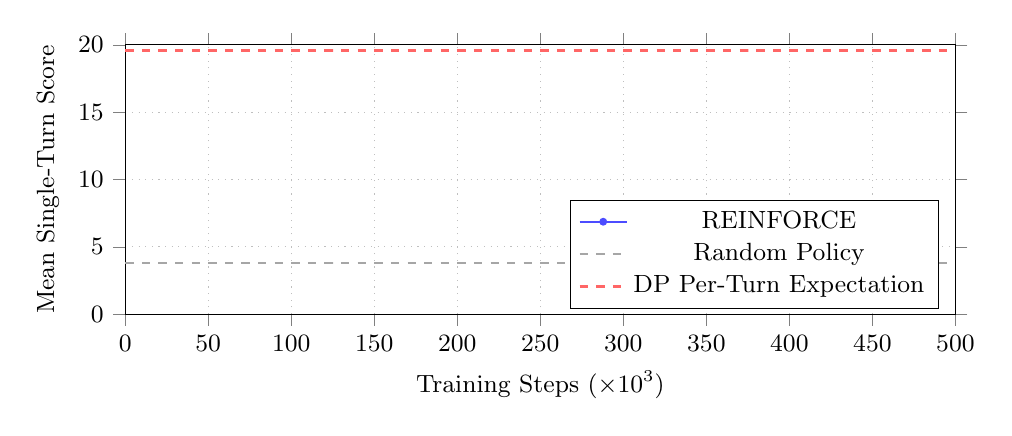
\begin{tikzpicture}
        \begin{axis}[
                width=\columnwidth,
                height=5cm,
                xlabel={Training Steps ($\times 10^3$)},
                ylabel={Mean Single-Turn Score},
                xmin=0, xmax=500,
                ymin=0, ymax=20,
                grid=both,
                grid style={dotted},
                tick align=outside,
                tick label style={font=\small},
                label style={font=\small},
                legend style={at={(0.98,0.02)},anchor=south east,font=\small}
            ]

            % Main REINFORCE learning curve
            \addplot[
                thick,
                blue!70!white,
                mark=*,
                mark size=1pt,
                mark repeat=10
            ] coordinates {
                    (0, 50)
                    (50, 50)
                    (100, 50)
                    (150, 50)
                    (200, 50)
                    (250, 50)
                    (300, 50)
                    (350, 50)
                    (400, 50)
                    (450, 50)
                    (500, 50)
                };
            \addlegendentry{REINFORCE}

            % Random policy baseline
            \addplot[
                dashed,
                gray!70,
                thick,
                domain=0:500
            ] {3.8};
            \addlegendentry{Random Policy}

            % DP per-turn expectation
            \addplot[
                dashed,
                red!60!white,
                thick,
                domain=0:500
            ] {19.59};
            \addlegendentry{DP Per-Turn Expectation}

        \end{axis}
    \end{tikzpicture}
    \caption{Single-turn agent performance during training (placeholder data)}
    \label{fig:single-turn-performance}
\end{figure}


\begin{figure}[b]
    \centering
    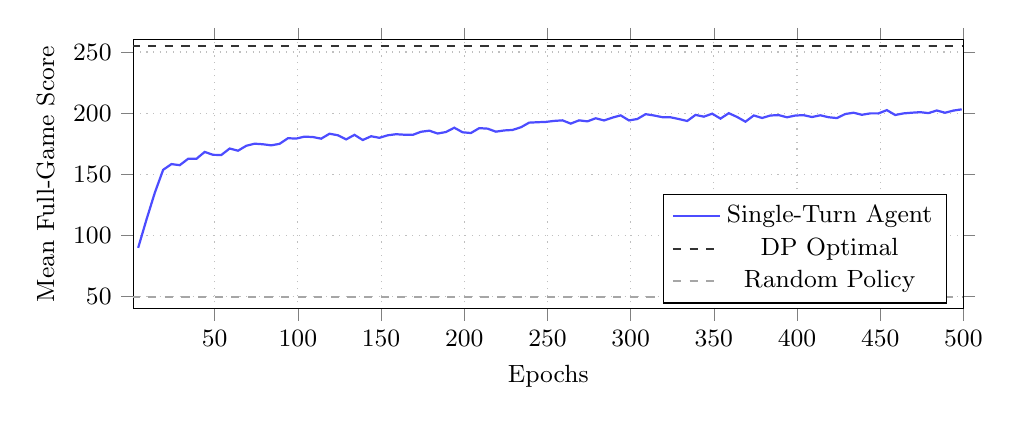
\begin{tikzpicture}
        \begin{axis}[
                width=\columnwidth,
                height=5cm,
                xlabel={Epochs},
                ylabel={Mean Full-Game Score},
                xmin=1, xmax=500,
                ymin=40, ymax=260,
                grid=both,
                grid style={dotted},
                tick align=outside,
                tick label style={font=\small},
                label style={font=\small},
                legend style={at={(0.98,0.02)},anchor=south east,font=\small}
            ]

            % Full-game evaluation at checkpoints
            \addplot[
                thick,
                blue!70!white
            ] coordinates {
                    (4, 89.93699646)
                    (9, 113.0670013)
                    (14, 134.9360046)
                    (19, 153.6799927)
                    (24, 158.3769989)
                    (29, 157.4949951)
                    (34, 162.6779938)
                    (39, 162.6869965)
                    (44, 168.3280029)
                    (49, 165.9459991)
                    (54, 165.8280029)
                    (59, 171.1269989)
                    (64, 169.3150024)
                    (69, 173.3609924)
                    (74, 175.0670013)
                    (79, 174.5850067)
                    (84, 173.7129974)
                    (89, 174.9400024)
                    (94, 179.522995)
                    (99, 179.2380066)
                    (104, 180.8220062)
                    (109, 180.496994)
                    (114, 179.1670074)
                    (119, 183.1909943)
                    (124, 181.9689941)
                    (129, 178.5579987)
                    (134, 182.2749939)
                    (139, 178.0599976)
                    (144, 181.1329956)
                    (149, 179.8670044)
                    (154, 181.9250031)
                    (159, 182.7960052)
                    (164, 182.3899994)
                    (169, 182.2640076)
                    (174, 184.8040009)
                    (179, 185.6869965)
                    (184, 183.3809967)
                    (189, 184.5890045)
                    (194, 188.1130066)
                    (199, 184.3699951)
                    (204, 183.7799988)
                    (209, 187.7700043)
                    (214, 187.3439941)
                    (219, 184.8800049)
                    (224, 185.878006)
                    (229, 186.2769928)
                    (234, 188.4429932)
                    (239, 192.2519989)
                    (244, 192.6029968)
                    (249, 192.8509979)
                    (254, 193.6679993)
                    (259, 194.1340027)
                    (264, 191.4689941)
                    (269, 194.1349945)
                    (274, 193.3059998)
                    (279, 195.8390045)
                    (284, 194.0599976)
                    (289, 196.3509979)
                    (294, 198.201004)
                    (299, 194.0650024)
                    (304, 195.2200012)
                    (309, 199.1909943)
                    (314, 198.1199951)
                    (319, 196.7449951)
                    (324, 196.6300049)
                    (329, 195.1990051)
                    (334, 193.598999)
                    (339, 198.5839996)
                    (344, 197.1459961)
                    (349, 199.5839996)
                    (354, 195.5440063)
                    (359, 199.9980011)
                    (364, 196.8760071)
                    (369, 193.048996)
                    (374, 198.1450043)
                    (379, 196.0639954)
                    (384, 198.1000061)
                    (389, 198.4129944)
                    (394, 196.6179962)
                    (399, 198.0950012)
                    (404, 198.348999)
                    (409, 196.848999)
                    (414, 198.2680054)
                    (419, 196.6640015)
                    (424, 195.9869995)
                    (429, 199.3150024)
                    (434, 200.3540039)
                    (439, 198.6880035)
                    (444, 199.8220062)
                    (449, 199.8170013)
                    (454, 202.4900055)
                    (459, 198.5119934)
                    (464, 199.8170013)
                    (469, 200.3809967)
                    (474, 200.8209991)
                    (479, 200.0529938)
                    (484, 202.1959991)
                    (489, 200.348999)
                    (494, 202.1139984)
                    (499, 203.1260071)
                };
            \addlegendentry{Single-Turn Agent}

            % DP optimal baseline
            \addplot[
                dashed,
                black!80,
                thick,
                domain=0:500
            ] {254.69};
            \addlegendentry{DP Optimal}

            % Random policy baseline
            \addplot[
                dashed,
                gray!70,
                thick,
                domain=0:500
            ] {49.5};
            \addlegendentry{Random Policy}

        \end{axis}
    \end{tikzpicture}
    \caption{Full-game performance of single-turn agent}
    \label{fig:single-turn-fullgame}
\end{figure}


\subsubsection{Single vs Full-game Tradeoff Curve}
\label{sec:tradeoff-curve}
To understand the tradeoff between single-turn and full-game performance, we ablated our model using small changes to various hyperparameters and captured
the resulting performance on both the primary single-turn score, as well as the auxiliary full-game score.
We expect that there is a Pareto frontier between these two objectives, and that some hyperparameter choices push performance towards one or the other.

As expected, we can see that full game performance generally increases linearly with single-turn performance.
However, at very high levels of full-game performance, single-turn performance begins to plateau, and even decline slightly.
Since the single-turn model does not have access to the full game context, these are actually imperfectly optimizing their purported objective.
This indicates that selecting hyperparameters for a single-turn model based on full-game performance could indeed be a form of target leakage.

\begin{figure}[htb]
    \centering
    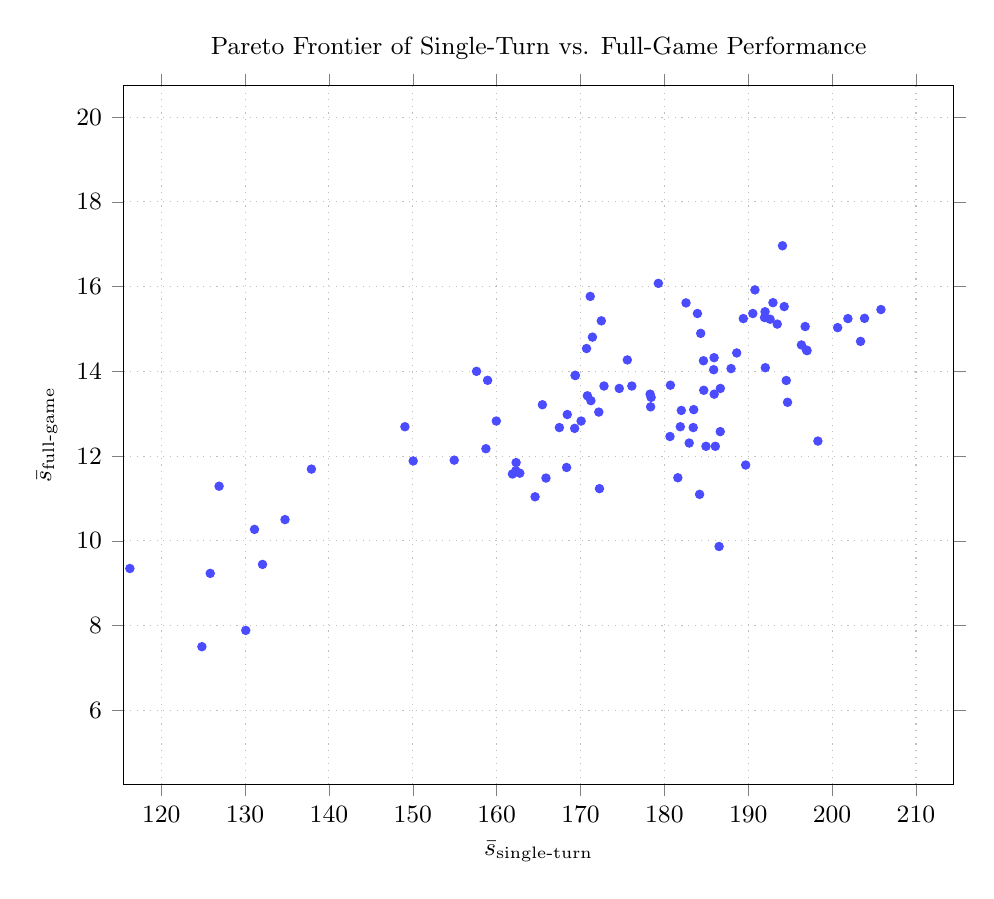
\begin{tikzpicture}
        \begin{axis}[
            width=\columnwidth,
            xlabel={$\bar{s}_{\text{single-turn}}$},
            ylabel={$\bar{s}_{\text{full-game}}$},
            title={Pareto Frontier of Single-Turn vs. Full-Game Performance},
            grid=both,
            grid style={dotted},
            tick align=outside,
            tick label style={font=\small},
            label style={font=\small},
            title style={font=\small},
            enlargelimits=0.05,
            xmin=120,
            xmax=210,
            ymin=5,
            ymax=20
            ]

            \addplot[
                only marks,
                mark=*,
                blue!70!white,
                mark size=1.5pt
            ] coordinates {
                    (184.3300018310547,14.89645004272461)
                    (200.66400146484375,15.032544136047363)
                    (203.3939971923828,14.707100868225098)
                    (201.8860015869141,15.245562553405762)
                    (194.53500366210935,13.784024238586426)
                    (205.8249969482422,15.45884609222412)
                    (192.947998046875,15.621301651000977)
                    (203.8679962158203,15.251479148864746)
                    (189.41200256347656,15.245562553405762)
                    (184.69500732421875,13.553255081176758)
                    (196.94400024414065,14.502958297729492)
                    (192.03700256347656,14.08579921722412)
                    (196.78900146484375,15.057692527770996)
                    (197.01499938964844,14.488165855407717)
                    (194.0850067138672,16.964496612548828)
                    (188.6269989013672,14.434171676635742)
                    (196.3419952392578,14.623077392578123)
                    (187.9499969482422,14.065089225769045)
                    (194.2899932861328,15.528846740722656)
                    (170.07000732421875,12.826923370361328)
                    (192.0070037841797,15.406805038452148)
                    (165.4550018310547,13.211539268493652)
                    (190.5449981689453,15.365385055541992)
                    (193.45899963378903,15.115385055541992)
                    (184.96099853515625,12.230770111083984)
                    (189.69400024414065,11.788461685180664)
                    (192.6060028076172,15.230770111083984)
                    (178.36000061035156,13.162307739257812)
                    (183.44000244140625,12.673077583312988)
                    (186.07400512695312,12.230770111083984)
                    (186.5260009765625,9.865385055541992)
                    (137.90899658203125,11.69230842590332)
                    (131.1219940185547,10.269230842590332)
                    (125.84300231933594,9.230769157409668)
                    (132.0780029296875,9.44230842590332)
                    (150.04800415039062,11.884615898132324)
                    (185.8780059814453,14.038461685180664)
                    (191.94200134277344,15.269231796264648)
                    (185.927001953125,14.322484970092772)
                    (194.68499755859375,13.269230842590332)
                    (186.6719970703125,13.59615421295166)
                    (124.85199737548828,7.500000476837158)
                    (186.6629943847656,12.576923370361328)
                    (180.67100524902344,12.461539268493652)
                    (184.10400390625,3.538461685180664)
                    (181.60499572753903,11.488165855407717)
                    (198.3070068359375,12.353846549987791)
                    (193.4470062255859,1.519230842590332)
                    (183.07000732421875,23.615385055541992)
                    (169.36000061035156,13.903846740722656)
                    (168.33999633789062,11.730770111083984)
                    (171.4199981689453,14.807692527770996)
                    (170.72000122070312,14.538461685180664)
                    (182.02000427246097,13.076923370361328)
                    (171.24000549316406,13.307692527770996)
                    (181.8999938964844,12.69230842590332)
                    (182.9600067138672,12.307692527770996)
                    (190.8000030517578,15.923076629638672)
                    (171.16000366210938,15.769230842590332)
                    (169.3800048828125,13.90384578704834)
                    (178.4199981689453,13.384614944458008)
                    (176.1199951171875,13.65384578704834)
                    (175.5800018310547,14.269230842590332)
                    (185.94000244140625,13.461538314819336)
                    (179.27999877929688,16.076923370361328)
                    (168.4199981689453,12.980769157409668)
                    (183.94000244140625,15.365385055541992)
                    (169.3000030517578,12.65384578704834)
                    (172.47999572753906,15.192307472229004)
                    (178.3000030517578,13.461538314819336)
                    (183.5,13.09615421295166)
                    (180.72000122070312,13.673076629638672)
                    (184.66000366210935,14.25)
                    (167.47999572753906,12.673076629638672)
                    (158.9199981689453,13.788461685180664)
                    (182.5800018310547,15.615385055541992)
                    (184.1999969482422,11.09615421295166)
                    (172.8000030517578,13.65384578704834)
                    (170.82000732421875,13.423076629638672)
                    (130.0800018310547,7.884615421295166)
                    (165.8800048828125,11.480769157409668)
                    (172.17999267578125,13.038461685180664)
                    (174.6199951171875,13.59615421295166)
                    (75.22000122070312,5.67307710647583)
                    (162.75999450683594,11.59615421295166)
                    (164.5800018310547,11.038461685180664)
                    (172.25999450683594,11.230769157409668)
                    (149.05999755859375,12.692307472229004)
                    (157.60000610351562,14)
                    (158.72000122070312,12.173076629638672)
                    (154.94000244140625,11.90384578704834)
                    (162.32000732421875,11.84615421295166)
                    (162.27999877929688,11.65384578704834)
                    (161.8800048828125,11.576923370361328)
                    (134.75999450683594,10.5)
                    (159.9600067138672,12.826923370361328)
                    (126.9000015258789,11.288461685180664)
                    (116.26000213623048,9.34615421295166)
                    (101.26000213623048,13.576923370361328)
                    (78.44000244140625,13)
                    (68.27999877929688,9.769230842590332)
                    (72,13.769230842590332)
                    (62.040000915527344,13.75)
                    (62.540000915527344,10.769230842590332)
                    (64.76000213623047,12.269230842590332)
                    (80.83999633789062,10.423076629638672)
                    (77.91999816894531,11.788461685180664)
                    (64.31999969482422,7.82692289352417)
                    (101.05999755859376,12.019230842590332)
                    (70.13999938964844,10.09615421295166)
                    (80.22000122070312,10.269230842590332)
                    (86.5199966430664,13.038461685180664)
                    (58.900001525878906,7.67307710647583)
                    (58.060001373291016,10.192307472229004)
                    (71.05999755859375,9.326923370361328)
                    (65.86000061035156,7.980769157409668)
                    (65.33999633789062,9.711538314819336)
                    (69.45999908447266,10.634614944458008)
                    (65.54000091552734,12.557692527770996)
                    (94.0199966430664,15.057692527770996)
                    (54.5,8.365385055541992)
                    (64.19999694824219,7.096153736114502)
                    (65.05999755859375,10.230769157409668)
                    (76.22000122070312,9.788461685180664)
                    (95.4000015258789,14.538461685180664)
                    (68.41999816894531,8.557692527770996)
                    (73.45999908447266,9.807692527770996)
                    (71.68000030517578,9.230769157409668)
                    (61.279998779296875,8.288461685180664)
                    (97.12000274658205,11.192307472229004)
                    (73.04000091552734,9.711538314819336)
                    (75.4800033569336,12.615385055541992)
                    (69.54000091552734,9.076923370361328)
                    (99.4800033569336,12.038461685180664)
                    (92.36000061035156,12.861538887023926)
                    (102.3000030517578,12.29230785369873)
                    (99.44000244140624,15.36923122406006)
                    (78.0999984741211,10.025641441345217)
                    (55.560001373291016,5.711538314819336)
                    (62.18000030517578,8.34615421295166)
                    (104.31999969482422,13.576923370361328)
                    (52.36000061035156,8.038461685180664)
                    (101.9800033569336,13.788461685180664)
                    (58.86000061035156,8.769230842590332)
                    (77.30000305175781,11.36923122406006)
                    (99,12.461538314819336)
                    (82.4800033569336,12.41538429260254)
                    (105.66000366210938,13.019230842590332)
                    (96.5999984741211,15.923076629638672)
                    (62.58000183105469,8.788461685180664)
                    (96.5999984741211,13.423076629638672)
                    (105.0199966430664,14.769230842590332)
                    (104.8000030517578,14.730769157409668)
                    (50.70000076293945,4.538461685180664)
                    (76.63999938964844,11.230769157409668)
                    (93.66000366210938,13.115385055541992)
                    (98.05999755859376,14.019230842590332)
                    (109.05999755859376,15.019230842590332)
                    (98.58000183105467,13.461538314819336)
                    (91.4800033569336,12.025641441345217)
                    (61.400001525878906,6.512820720672607)
                    (54.31999969482422,7.641025543212891)
                    (89.5,14.076923370361328)
                    (58.900001525878906,11.538461685180664)
                    (87.5999984741211,10.64102554321289)
                    (59.720001220703125,8.326923370361328)
                    (59.040000915527344,7.942307472229004)
                    (83.30000305175781,12.288461685180664)
                    (54.79999923706055,8.461538314819336)
                    (52.13999938964844,6.512820720672607)
                    (107.58000183105467,10.820512771606444)
                    (60.02000045776367,8.480769157409668)
                    (57.279998779296875,6.75)
                    (78.9000015258789,11.75)
                    (44.880001068115234,7.92307710647583)
                    (68.27999877929688,11.538461685180664)
                    (59.439998626708984,5.538461685180664)
                    (63.36000061035156,9.769230842590332)
                    (105.63999938964844,9.84615421295166)
                    (50.880001068115234,7.538461685180664)
                    (111.18000030517578,10.923076629638672)
                    (60.599998474121094,9.09615421295166)
                    (90.3000030517578,13.576923370361328)
                    (52.7599983215332,11.076923370361328)
                    (58.34000015258789,7.980769157409668)
                    (66.0999984741211,10.038461685180664)
                    (48.13999938964844,3.3333332538604736)
                    (106.5999984741211,15.051281929016112)
                    (70,9.923076629638672)
                    (38.63999938964844,4.461538314819336)
                    (66.4000015258789,5.92307710647583)
                    (90.4000015258789,13.34615421295166)
                    (63.31999969482422,10.423076629638672)
                    (56.70000076293945,6.42307710647583)
                    (89.37999725341797,9.974358558654783)
                    (52.86000061035156,8.84615421295166)
                    (33.91999816894531,4.807692527770996)
                    (60.08000183105469,9.333333015441896)
                    (80.16000366210938,8.769230842590332)
                    (53.86000061035156,5.333333492279053)
                    (109.68000030517578,14.90384578704834)
                    (61.779998779296875,10.307692527770996)
                    (45.959999084472656,8.34615421295166)
                    (97.58000183105467,11.230769157409668)
                    (55.279998779296875,9.384614944458008)
                    (53.7599983215332,9.307692527770996)
                    (51.81999969482422,11.461538314819336)
                    (67.91999816894531,6.769230842590332)
                    (93.76000213623048,15.743589401245115)
                    (72.44000244140625,9.615385055541992)
                    (47.439998626708984,6.692307472229004)
                    (50.7599983215332,6)
                    (93.68000030517578,11.423076629638672)
                };

        \end{axis}
    \end{tikzpicture}
    \caption{Single-turn vs full-game performance (placeholder data)}
    \label{fig:pareto-frontier}
\end{figure}

\subsection{Full-Game Results}
% <600-700 words>
For the full-game model, we added several additional features to the state representation: $\phi_{\mathrm{progress}}(t)$ and $\phi_{\mathrm{potential}}(\mathbf{d}, \mathbf{c})$
while reusing the same underlying neural network architecture as the single-turn model. These additions were necessary to provide the model with sufficient context to make long-term strategic decisions.
While the $\phi_{\mathrm{progress}}(t)$ feature could be inferred from the scorecard, the model struggled to do so reliably.
We intentionally omitted the $\phi_{\mathrm{potential}}(\mathbf{d}, \mathbf{c})$ feature in single turn, as we wanted to ensure the model was capable of learning to reason about category potential on its own,
but found it to be necessary, especially with REINFORCE.

\subsubsection{Algorithm Comparison: REINFORCE, A2C, PPO}

REINFORCE proved challenging to optimize to high performance levels given our fixed training budget of 1 million full-game episodes (39 million steps).
It was highly sensitive to hyperparameters such as the critic coefficient, the entropy bonus, and batch size.
We also found that REINFORCE simply required more training data to converge at a reliable performance level across seeds; our implementation was trained on 1,000,000 games.
However, after optimization we were able to achieve reasonable performance, scoring a mean of <X> points on average over 10,000 full games.

Our most successful algorithm was TD(0)-style Actor-Critic (A2C). We found is easiest to tune and with an immediate performance boost over REINFORCE.
This was the algorithm we use for the ablation studies. With a fixed training budget of 1 million full-games,
A2C was able to approach DP-optimal performance.

We also attempted to use Proximal Policy Optimization (PPO) with TD(0), but found it difficult to tune effectively within our computational budget. Each PPO rollout requires
$k$ epochs of minibatch updates, which significantly increases training time compared to A2C and REINFORCE. Sample efficiency wasn't a huge factor for us, since Yahtzee is so easy to simulate.
For fair comparison to the other algorithms, we had to reduce the total number of games seen during training by a factor of $k$.
However, it is possible PPO could reach or surpass A2C performance with more extensive hyperparameter tuning.

\begin{figure}[t]
  \centering
  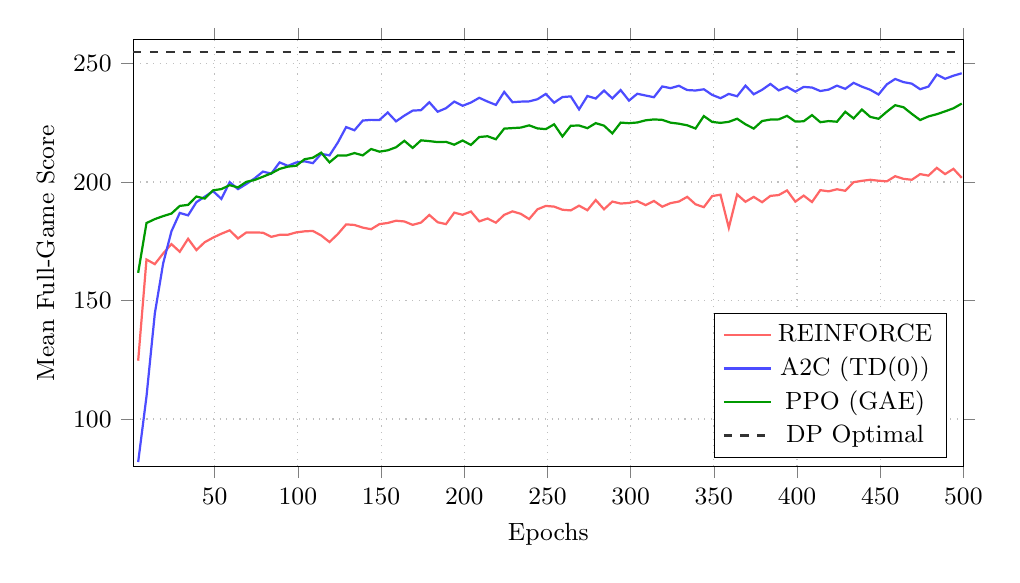
\begin{tikzpicture}
    \begin{axis}[
        width=\columnwidth,
        height=7cm,
        xlabel={Epochs},
        ylabel={Mean Full-Game Score},
        xmin=1, xmax=500,
        ymin=80, ymax=260,
        grid=both,
        grid style={dotted},
        tick align=outside,
        tick label style={font=\small},
        label style={font=\small},
        title style={font=\small},
        legend style={at={(0.98,0.02)},anchor=south east,font=\small}
      ]

      % REINFORCE learning curve
      \addplot[
        thick,
        red!60!white
      ] coordinates {
          (4, 124.59100341796875)
          (9, 167.27999877929688)
          (14, 165.33299255371094)
          (19, 169.83200073242188)
          (24, 173.79200744628906)
          (29, 170.5570068359375)
          (34, 176.0330047607422)
          (39, 171.27200317382812)
          (44, 174.5959930419922)
          (49, 176.51199340820312)
          (54, 178.1649932861328)
          (59, 179.58999633789062)
          (64, 176.1719970703125)
          (69, 178.7010040283203)
          (74, 178.71400451660156)
          (79, 178.5919952392578)
          (84, 176.8470001220703)
          (89, 177.6959991455078)
          (94, 177.7449951171875)
          (99, 178.7259979248047)
          (104, 179.1719970703125)
          (109, 179.3439941)
          (114, 177.42799377441406)
          (119, 174.65699768066406)
          (124, 178.0330047607422)
          (129, 182.1020050048828)
          (134, 181.87100219726562)
          (139, 180.73899841308594)
          (144, 180.0659942626953)
          (149, 182.21600341796875)
          (154, 182.69700622558594)
          (159, 183.65199279785156)
          (164, 183.3439941)
          (169, 181.90499877929688)
          (174, 182.86199951171875)
          (179, 186.08399963378906)
          (184, 183.01400756835938)
          (189, 182.2189941)
          (194, 187.06399536132812)
          (199, 186.16600036621094)
          (204, 187.53599548339844)
          (209, 183.38499450683594)
          (214, 184.58299255371094)
          (219, 182.82000732421875)
          (224, 186.12600708007812)
          (229, 187.5970001220703)
          (234, 186.55499267578125)
          (239, 184.35000610351562)
          (244, 188.47500610351562)
          (249, 189.8959961)
          (254, 189.60899353027344)
          (259, 188.27999877929688)
          (264, 188.00999450683594)
          (269, 190.00100708007812)
          (274, 188.08099365234375)
          (279, 192.38600158691406)
          (284, 188.48199462890625)
          (289, 191.7259979248047)
          (294, 190.89999389648438)
          (299, 191.14300537109375)
          (304, 191.9250030517578)
          (309, 190.24400329589844)
          (314, 191.99200439453125)
          (319, 189.5709991455078)
          (324, 191.08200073242188)
          (329, 191.7469940185547)
          (334, 193.72799682617188)
          (339, 190.5780029296875)
          (344, 189.36700439453125)
          (349, 194.0570068359375)
          (354, 194.63299560546875)
          (359, 180.67999267578125)
          (364, 194.74099731445312)
          (369, 191.6439971923828)
          (374, 193.70899963378906)
          (379, 191.4689941)
          (384, 194.13499450683594)
          (389, 194.4770050048828)
          (394, 196.43800354003906)
          (399, 191.697998)
          (404, 194.24099731445312)
          (409, 191.5399932861328)
          (414, 196.55599975585938)
          (419, 196.04200744628906)
          (424, 196.9320068359375)
          (429, 196.2779998779297)
          (434, 199.91400146484375)
          (439, 200.48500061035156)
          (444, 200.927002)
          (449, 200.5310059)
          (454, 200.2729949951172)
          (459, 202.43299865722656)
          (464, 201.31700134277344)
          (469, 200.92599487304688)
          (474, 203.3070068359375)
          (479, 202.6909942626953)
          (484, 205.95599365234375)
          (489, 203.32200622558594)
          (494, 205.53799438476562)
          (499, 201.76300048828125)
        };
      \addlegendentry{REINFORCE}

      % A2C learning curve
      \addplot[
        thick,
        blue!70!white
      ] coordinates {
          (4, 81.84799957)
          (9, 109.50599670410156)
          (14, 144.4689941)
          (19, 165.6179962158203)
          (24, 179.17999267578125)
          (29, 186.93899536132812)
          (34, 185.91200256347656)
          (39, 191.47500610351562)
          (44, 193.7790069580078)
          (49, 196.1540069580078)
          (54, 192.8699951171875)
          (59, 199.93600463867188)
          (64, 196.98599243164062)
          (69, 199.1300048828125)
          (74, 201.5229949951172)
          (79, 204.38400268554688)
          (84, 203.5189971923828)
          (89, 208.25999450683594)
          (94, 206.802002)
          (99, 208.22999572753906)
          (104, 208.7189941)
          (109, 207.94200134277344)
          (114, 211.8820037841797)
          (119, 211.2169952392578)
          (124, 216.63600158691406)
          (129, 223.1510009765625)
          (134, 221.8209991455078)
          (139, 225.91799926757812)
          (144, 226.1999969482422)
          (149, 226.1490020751953)
          (154, 229.30799865722656)
          (159, 225.5850067138672)
          (164, 228.0019989013672)
          (169, 230.10299682617188)
          (174, 230.3040008544922)
          (179, 233.63900756835938)
          (184, 229.63800048828125)
          (189, 231.11700439453125)
          (194, 233.9250030517578)
          (199, 232.13900756835938)
          (204, 233.51600646972656)
          (209, 235.51199340820312)
          (214, 233.92300415039062)
          (219, 232.51699829101562)
          (224, 238.00399780273438)
          (229, 233.65899658203125)
          (234, 233.89700317382812)
          (239, 233.99899291992188)
          (244, 234.9080047607422)
          (249, 237.14300537109375)
          (254, 233.44400024414062)
          (259, 235.8249969482422)
          (264, 236.1009979248047)
          (269, 230.63699340820312)
          (274, 236.27200317382812)
          (279, 235.21299743652344)
          (284, 238.56500244140625)
          (289, 235.25799560546875)
          (294, 238.7469940185547)
          (299, 234.33399963378906)
          (304, 237.2220001220703)
          (309, 236.4709930419922)
          (314, 235.7550048828125)
          (319, 240.2989959716797)
          (324, 239.58099365234375)
          (329, 240.58099365234375)
          (334, 238.7790069580078)
          (339, 238.59100341796875)
          (344, 239.10499572753906)
          (349, 236.74200439453125)
          (354, 235.3350067138672)
          (359, 237.1479949951172)
          (364, 236.16000366210938)
          (369, 240.6219940185547)
          (374, 237.00799560546875)
          (379, 238.88499450683594)
          (384, 241.3520050048828)
          (389, 238.63999938964844)
          (394, 240.12899780273438)
          (399, 238.10800170898438)
          (404, 240.10899353027344)
          (409, 239.83900451660156)
          (414, 238.3679962158203)
          (419, 238.96299743652344)
          (424, 240.63400268554688)
          (429, 239.28500366210938)
          (434, 241.82200622558594)
          (439, 240.20799255371094)
          (444, 238.89999389648438)
          (449, 236.9010009765625)
          (454, 241.19700622558594)
          (459, 243.45399475097656)
          (464, 242.12899780273438)
          (469, 241.48599243164062)
          (474, 239.13499450683594)
          (479, 240.2519989013672)
          (484, 245.30799865722656)
          (489, 243.5290069580078)
          (494, 244.82899475097656)
          (499, 245.86099243164062)
        };
      \addlegendentry{A2C (TD(0))}

      % PPO learning curve
      \addplot[
        thick,
        green!60!black
      ] coordinates {
          (4, 161.6560059)
          (9, 182.66700744628906)
          (14, 184.33399963378906)
          (19, 185.5959930419922)
          (24, 186.6790008544922)
          (29, 189.8979949951172)
          (34, 190.33900451660156)
          (39, 193.86399841308594)
          (44, 192.99899291992188)
          (49, 196.4739990234375)
          (54, 197.00100708007812)
          (59, 198.64700317382812)
          (64, 197.7239990234375)
          (69, 200.05599975585938)
          (74, 200.8489990234375)
          (79, 202.22000122070312)
          (84, 203.63299560546875)
          (89, 205.50999450683594)
          (94, 206.47500610351562)
          (99, 206.8459930419922)
          (104, 209.58599853515625)
          (109, 210.2310028076172)
          (114, 212.37399291992188)
          (119, 208.2760009765625)
          (124, 211.1959991455078)
          (129, 211.12600708007812)
          (134, 212.19700622558594)
          (139, 211.2270050048828)
          (144, 213.90899658203125)
          (149, 212.79299926757812)
          (154, 213.3470001220703)
          (159, 214.6510009765625)
          (164, 217.36399841308594)
          (169, 214.3679962158203)
          (174, 217.5679931640625)
          (179, 217.23300170898438)
          (184, 216.82899475097656)
          (189, 216.9250030517578)
          (194, 215.7259979248047)
          (199, 217.4929962158203)
          (204, 215.61700439453125)
          (209, 218.97500610351562)
          (214, 219.28900146484375)
          (219, 218.01800537109375)
          (224, 222.50900268554688)
          (229, 222.72799682617188)
          (234, 222.9459991455078)
          (239, 223.88600158691406)
          (244, 222.59500122070312)
          (249, 222.29800415039062)
          (254, 224.3260040283203)
          (259, 219.20199584960938)
          (264, 223.70899963378906)
          (269, 223.83999633789062)
          (274, 222.69500732421875)
          (279, 224.8249969482422)
          (284, 223.76499938964844)
          (289, 220.49099731445312)
          (294, 225.04299926757812)
          (299, 224.80599975585938)
          (304, 225.0959930419922)
          (309, 226.01400756835938)
          (314, 226.38900756835938)
          (319, 226.20399475097656)
          (324, 225.02699279785156)
          (329, 224.58700561523438)
          (334, 223.91299438476562)
          (339, 222.5540008544922)
          (344, 227.80799865722656)
          (349, 225.33099365234375)
          (354, 224.92799377441406)
          (359, 225.3769989013672)
          (364, 226.6820068359375)
          (369, 224.33700561523438)
          (374, 222.53399658203125)
          (379, 225.71099853515625)
          (384, 226.3300018310547)
          (389, 226.40899658203125)
          (394, 227.89500427246094)
          (399, 225.48800659179688)
          (404, 225.6009979248047)
          (409, 228.20700073242188)
          (414, 225.2169952392578)
          (419, 225.6909942626953)
          (424, 225.41900634765625)
          (429, 229.61300659179688)
          (434, 226.822998)
          (439, 230.5500030517578)
          (444, 227.46499633789062)
          (449, 226.65899658203125)
          (454, 229.66000366210938)
          (459, 232.3939971923828)
          (464, 231.5189971923828)
          (469, 228.72799682617188)
          (474, 226.13600158691406)
          (479, 227.64999389648438)
          (484, 228.5970001220703)
          (489, 229.79200744628906)
          (494, 231.0780029296875)
          (499, 233.0749969482422)
        };
      \addlegendentry{PPO (GAE)}

      % DP optimal baseline
      \addplot[
        dashed,
        black!80,
        thick,
        domain=1:500
      ] {254.69};
      \addlegendentry{DP Optimal}

    \end{axis}
  \end{tikzpicture}
  \caption{Full-Game Learning Curves by Algorithm}
  \label{fig:full-game-learning-curves}
\end{figure}

\begin{figure}[t]
    \centering
    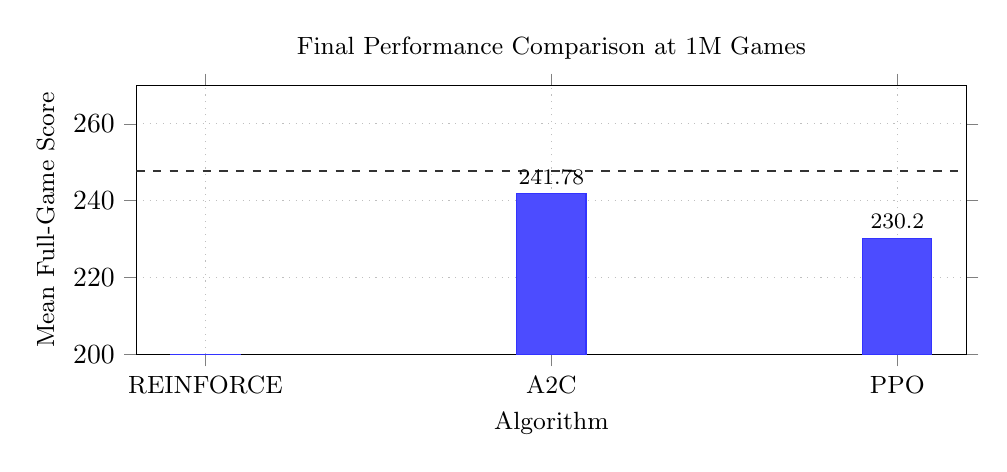
\begin{tikzpicture}
        \begin{axis}[
                ybar,
                width=\columnwidth,
                height=5cm,
                xlabel={Algorithm},
                ylabel={Mean Full-Game Score},
                title={Final Performance Comparison at 1M Games},
                symbolic x coords={REINFORCE, A2C, PPO, DP Optimal},
                xtick=data,
                xticklabel style={font=\small},
                ylabel style={font=\small},
                xlabel style={font=\small},
                title style={font=\small},
                bar width=25pt,
                ymin=200, ymax=270,
                grid=both,
                grid style={dotted},
                tick align=outside,
                nodes near coords,
                nodes near coords style={font=\footnotesize, anchor=south},
            ]

            \addplot[
                fill=blue!70!white,
                draw=blue!80,
                error bars/.cd,
                y dir=both,
                y explicit
            ] coordinates {
                    (REINFORCE, 50)
                    (A2C, 241.78)
                    (PPO, 230.20)
                };

            % Horizontal dashed line at DP optimal spanning entire graph
            \draw[dashed, black!80, thick] (rel axis cs:0,0.682) -- (rel axis cs:1,0.682);

        \end{axis}
    \end{tikzpicture}
    \caption{Final performance, mean score}
    \label{fig:final-performance-comparison}
\end{figure}

\begin{figure}[b]
    \centering
    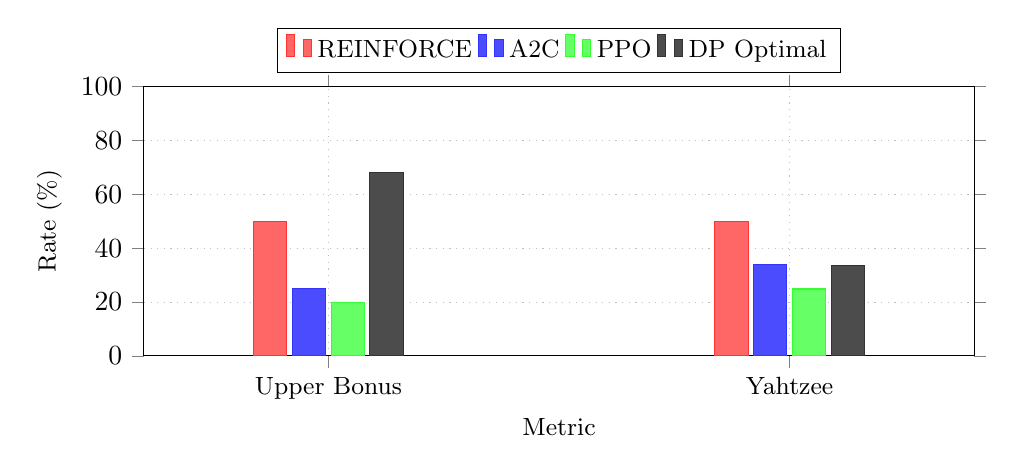
\begin{tikzpicture}
        \begin{axis}[
                ybar,
                width=\columnwidth,
                height=5cm,
                xlabel={Metric},
                ylabel={Rate (\%)},
                title={Bonus and Yahtzee Rates by Algorithm},
                symbolic x coords={Upper Bonus, Yahtzee},
                xtick=data,
                xticklabel style={font=\small},
                ylabel style={font=\small},
                xlabel style={font=\small},
                title style={font=\small},
                ymin=0, ymax=100,
                bar width=12pt,
                grid=both,
                grid style={dotted},
                tick align=outside,
                legend style={at={(0.5,1.05)},anchor=south,legend columns=4,font=\small},
                enlarge x limits=0.4,
            ]

            % REINFORCE
            \addplot[
                fill=red!60!white,
                draw=red!80!white
            ] coordinates {
                    (Upper Bonus, 50)
                    (Yahtzee, 50)
                };
            \addlegendentry{REINFORCE}

            % A2C
            \addplot[
                fill=blue!70!white,
                draw=blue!80!white
            ] coordinates {
                    (Upper Bonus, 24.93)
                    (Yahtzee, 34.05)
                };
            \addlegendentry{A2C}

            % PPO
            \addplot[
                fill=green!60!white,
                draw=green!80!white
            ] coordinates {
                    (Upper Bonus, 19.71)
                    (Yahtzee, 24.87)
                };
            \addlegendentry{PPO}

            % DP Optimal
            \addplot[
                fill=black!70,
                draw=black!80
            ] coordinates {
                    (Upper Bonus, 68.12)
                    (Yahtzee, 33.74)
                };
            \addlegendentry{DP Optimal}

        \end{axis}
    \end{tikzpicture}
    \caption{Bonus and Yahtzee achievement rates (placeholder data)}
    \label{fig:bonus-yahtzee-rates}
\end{figure}

\subsubsection{Representational Ablations}

While a number of additional representational choices were explored, one of the most important is the state representation of the dice.
One important thing to note is that our environment always sorts the dice in ascending order before passing them to the agent.
If this was not done, the network would be forced to waste capacity on understanding permutations of the same dice configuration,
which we found early on was a significant impediment to learning.

We wanted to highlight the importance of using a combined representation of both one-hot encodings and counts-based encodings of the dice.
While the network could theoretically learn to reconstruct either representation from the other, in practice we found that using both improved performance.

\begin{figure}[t]
    \centering
    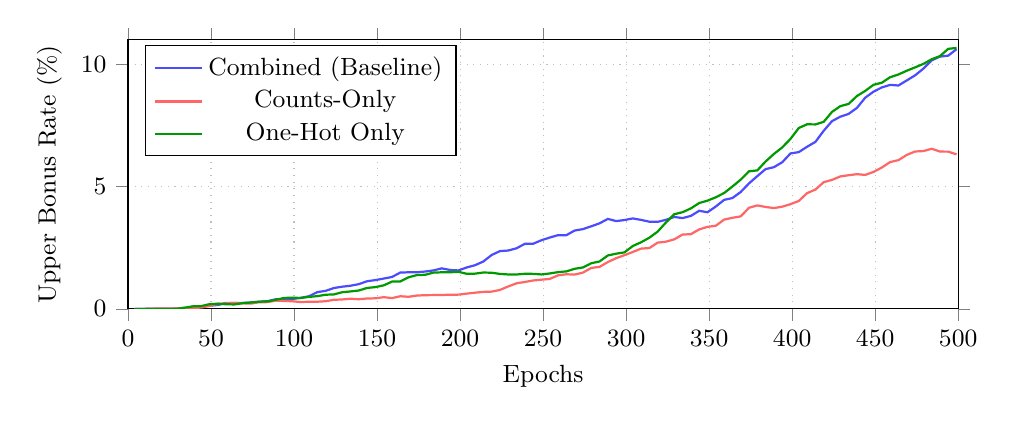
\begin{tikzpicture}
        \begin{axis}[
                width=\columnwidth,
                height=5cm,
                xlabel={Epochs},
                ylabel={Upper Bonus Rate (\%)},
                xmin=0, xmax=500,
                ymin=0, ymax=11,
                grid=both,
                grid style={dotted},
                tick align=outside,
                tick label style={font=\small},
                label style={font=\small},
                legend style={at={(0.02,0.98)},anchor=north west,font=\small}
            ]

            % Combined (desert-sweep-1)
            \addplot[
                thick,
                blue!70!white
            ] coordinates {
                    (4, 0)
                    (9, 0)
                    (14, 0.009)
                    (19, 0.0081)
                    (24, 0.00729)
                    (29, 0.016561)
                    (34, 0.0149049)
                    (39, 0.093414411)
                    (44, 0.104072971)
                    (49, 0.133665674)
                    (54, 0.160299107)
                    (59, 0.244269197)
                    (64, 0.239842277)
                    (69, 0.245858051)
                    (74, 0.261272246)
                    (79, 0.295145024)
                    (84, 0.315630522)
                    (89, 0.394067472)
                    (94, 0.404660725)
                    (99, 0.404194653)
                    (104, 0.453775185)
                    (109, 0.518397669)
                    (114, 0.686557907)
                    (119, 0.737902121)
                    (124, 0.854111906)
                    (129, 0.908700725)
                    (134, 0.94783066)
                    (139, 1.013047596)
                    (144, 1.131742841)
                    (149, 1.17856856)
                    (154, 1.240711699)
                    (159, 1.306640527)
                    (164, 1.485976464)
                    (169, 1.49737882)
                    (174, 1.497640938)
                    (179, 1.52787684)
                    (184, 1.575089156)
                    (189, 1.65758025)
                    (194, 1.591822225)
                    (199, 1.572640012)
                    (204, 1.69537603)
                    (209, 1.785838441)
                    (214, 1.937254592)
                    (219, 2.203529123)
                    (224, 2.363176206)
                    (229, 2.3868586)
                    (234, 2.478172735)
                    (239, 2.660355481)
                    (244, 2.664319937)
                    (249, 2.807887934)
                    (254, 2.91709915)
                    (259, 3.015389245)
                    (264, 3.01385032)
                    (269, 3.202465298)
                    (274, 3.262218763)
                    (279, 3.375996896)
                    (284, 3.498397197)
                    (289, 3.678557449)
                    (294, 3.590701723)
                    (299, 3.631631551)
                    (304, 3.698468415)
                    (309, 3.638621564)
                    (314, 3.564759393)
                    (319, 3.558283454)
                    (324, 3.642455118)
                    (329, 3.758209625)
                    (334, 3.712388658)
                    (339, 3.801149783)
                    (344, 4.011034814)
                    (349, 3.949931342)
                    (354, 4.184938227)
                    (359, 4.456444366)
                    (364, 4.530799958)
                    (369, 4.777719962)
                    (374, 5.12994789)
                    (379, 5.426953139)
                    (384, 5.714257749)
                    (389, 5.792831974)
                    (394, 5.993548796)
                    (399, 6.354193954)
                    (404, 6.408774521)
                    (409, 6.627897107)
                    (414, 6.825107434)
                    (419, 7.282596653)
                    (424, 7.674337064)
                    (429, 7.856903357)
                    (434, 7.971213022)
                    (439, 8.214091777)
                    (444, 8.632682561)
                    (449, 8.879414343)
                    (454, 9.051472851)
                    (459, 9.156325604)
                    (464, 9.130693101)
                    (469, 9.337623867)
                    (474, 9.543861442)
                    (479, 9.819475317)
                    (484, 10.15752777)
                    (489, 10.31177497)
                    (494, 10.35059745)
                    (499, 10.61553771)
                };
            \addlegendentry{Combined (Baseline)}

            % Counts-only (desert-sweep-2)
            \addplot[
                thick,
                red!60!white
            ] coordinates {
                    (4, 0)
                    (9, 0)
                    (14, 0.01)
                    (19, 0.019)
                    (24, 0.0171)
                    (29, 0.01539)
                    (34, 0.043851001)
                    (39, 0.039465901)
                    (44, 0.055519311)
                    (49, 0.119967385)
                    (54, 0.207970647)
                    (59, 0.227173582)
                    (64, 0.244456225)
                    (69, 0.230010603)
                    (74, 0.217009542)
                    (79, 0.275308589)
                    (84, 0.277777732)
                    (89, 0.339999956)
                    (94, 0.325999961)
                    (99, 0.313399965)
                    (104, 0.282059968)
                    (109, 0.293853972)
                    (114, 0.294468576)
                    (119, 0.315021719)
                    (124, 0.373519544)
                    (129, 0.38616759)
                    (134, 0.417550836)
                    (139, 0.395795752)
                    (144, 0.426216182)
                    (149, 0.433594564)
                    (154, 0.480235105)
                    (159, 0.442211595)
                    (164, 0.51799044)
                    (169, 0.496191397)
                    (174, 0.546572257)
                    (179, 0.561915036)
                    (184, 0.565723535)
                    (189, 0.569151184)
                    (194, 0.58223607)
                    (199, 0.584012466)
                    (204, 0.625611219)
                    (209, 0.663050097)
                    (214, 0.696745088)
                    (219, 0.70707058)
                    (224, 0.776363532)
                    (229, 0.918727183)
                    (234, 1.04685447)
                    (239, 1.102169025)
                    (244, 1.161952127)
                    (249, 1.195756915)
                    (254, 1.226181223)
                    (259, 1.373563106)
                    (264, 1.41620679)
                    (269, 1.404586118)
                    (274, 1.484127511)
                    (279, 1.67571477)
                    (284, 1.718143283)
                    (289, 1.91632896)
                    (294, 2.074696064)
                    (299, 2.197226453)
                    (304, 2.327503807)
                    (309, 2.464753431)
                    (314, 2.488278093)
                    (319, 2.709450265)
                    (324, 2.748505229)
                    (329, 2.843654711)
                    (334, 3.039289259)
                    (339, 3.055360337)
                    (344, 3.249824304)
                    (349, 3.354841892)
                    (354, 3.399357698)
                    (359, 3.649421938)
                    (364, 3.724479754)
                    (369, 3.782031798)
                    (374, 4.133828589)
                    (379, 4.230445721)
                    (384, 4.167401139)
                    (389, 4.12066103)
                    (394, 4.178594908)
                    (399, 4.280735446)
                    (404, 4.412661939)
                    (409, 4.731395736)
                    (414, 4.878256143)
                    (419, 5.180430586)
                    (424, 5.272387518)
                    (429, 5.415148795)
                    (434, 5.463633925)
                    (439, 5.507270542)
                    (444, 5.476543516)
                    (449, 5.598889193)
                    (454, 5.779000283)
                    (459, 6.001100255)
                    (464, 6.080990249)
                    (469, 6.292891205)
                    (474, 6.433602065)
                    (479, 6.450241849)
                    (484, 6.545217674)
                    (489, 6.430695916)
                    (494, 6.427626334)
                    (499, 6.314863672)
                };
            \addlegendentry{Counts-Only}

            % One-hot only (desert-sweep-3)
            \addplot[
                thick,
                green!60!black
            ] coordinates {
                    (4, 0)
                    (9, 0)
                    (14, 0)
                    (19, 0)
                    (24, 0)
                    (29, 0)
                    (34, 0.05)
                    (39, 0.105000002)
                    (44, 0.114500002)
                    (49, 0.19305)
                    (54, 0.213745)
                    (59, 0.1923705)
                    (64, 0.18313345)
                    (69, 0.23482011)
                    (74, 0.261338099)
                    (79, 0.295204292)
                    (84, 0.305683863)
                    (89, 0.375115477)
                    (94, 0.447603931)
                    (99, 0.462843541)
                    (104, 0.446559188)
                    (109, 0.491903267)
                    (114, 0.522712941)
                    (119, 0.580441649)
                    (124, 0.592397489)
                    (129, 0.68315774)
                    (134, 0.714841966)
                    (139, 0.753357772)
                    (144, 0.85802199)
                    (149, 0.892219796)
                    (154, 0.962997819)
                    (159, 1.116698037)
                    (164, 1.125028238)
                    (169, 1.292525433)
                    (174, 1.383272895)
                    (179, 1.394945605)
                    (184, 1.48545104)
                    (189, 1.496905938)
                    (194, 1.497215344)
                    (199, 1.517493815)
                    (204, 1.435744438)
                    (209, 1.442169994)
                    (214, 1.487952992)
                    (219, 1.479157703)
                    (224, 1.431241932)
                    (229, 1.408117744)
                    (234, 1.407305979)
                    (239, 1.436575386)
                    (244, 1.432917857)
                    (249, 1.409626076)
                    (254, 1.448663464)
                    (259, 1.503797117)
                    (264, 1.533417401)
                    (269, 1.640075675)
                    (274, 1.696068112)
                    (279, 1.866461311)
                    (284, 1.939815194)
                    (289, 2.185833684)
                    (294, 2.257250301)
                    (299, 2.31152529)
                    (304, 2.570372771)
                    (309, 2.723335484)
                    (314, 2.911001926)
                    (319, 3.159901743)
                    (324, 3.533911531)
                    (329, 3.870520339)
                    (334, 3.953468286)
                    (339, 4.108121458)
                    (344, 4.327309331)
                    (349, 4.424578369)
                    (354, 4.562120504)
                    (359, 4.735908472)
                    (364, 5.002317635)
                    (369, 5.28208589)
                    (374, 5.623877282)
                    (379, 5.661489554)
                    (384, 6.025340618)
                    (389, 6.332806499)
                    (394, 6.599525849)
                    (399, 6.949573302)
                    (404, 7.394615934)
                    (409, 7.545154398)
                    (414, 7.540639006)
                    (419, 7.646575143)
                    (424, 8.05191761)
                    (429, 8.286725906)
                    (434, 8.378053296)
                    (439, 8.700247909)
                    (444, 8.910223138)
                    (449, 9.159200786)
                    (454, 9.243280707)
                    (459, 9.468952636)
                    (464, 9.582057316)
                    (469, 9.733851622)
                    (474, 9.870466498)
                    (479, 10.01341987)
                    (484, 10.20207794)
                    (489, 10.33187014)
                    (494, 10.62868315)
                    (499, 10.66581483)
                };
            \addlegendentry{One-Hot Only}
        \end{axis}
    \end{tikzpicture}
    \caption{Exponential moving average (EMA) of upper-bonus achievement by dice representation}
    \label{fig:dice-representation-bonus}
\end{figure}


For the full-game model, we added several additional features beyond the single-turn representation.
To understand the importance of each, they were ablated individually.

\begin{figure}[b]
    \centering
    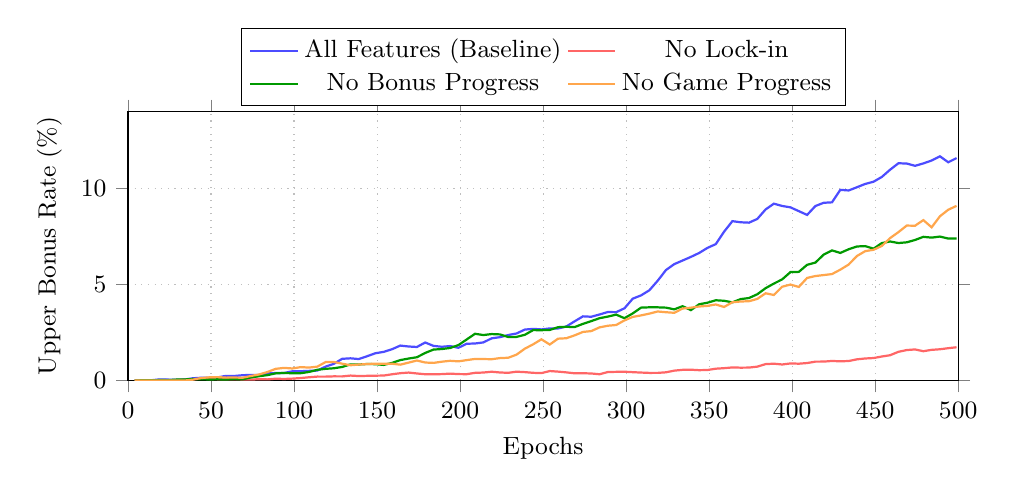
\begin{tikzpicture}
        \begin{axis}[
                width=\columnwidth,
                height=5cm,
                xlabel={Epochs},
                ylabel={Upper Bonus Rate (\%)},
                xmin=0, xmax=500,
                ymin=0, ymax=14,
                grid=both,
                grid style={dotted},
                tick align=outside,
                tick label style={font=\small},
                label style={font=\small},
                legend style={at={(0.5,1.02)},anchor=south,font=\small,legend columns=2}
            ]

            % All features (baseline)
            \addplot[
                thick,
                blue!70!white
            ] coordinates {
                    (4, 0) (9, 0) (14, 0.015) (19, 0.057750002) (24, 0.049087502) (29, 0.041724376) (34, 0.05046572) (39, 0.117895862) (44, 0.145211485) (49, 0.138429762) (54, 0.1626653) (59, 0.243265512) (64, 0.236775686) (69, 0.276259333) (74, 0.294820434) (79, 0.29559737) (84, 0.371257767) (89, 0.390569102) (94, 0.391983737) (99, 0.483186177) (104, 0.48570825) (109, 0.502852016) (114, 0.517424217) (119, 0.724810581) (124, 0.871089001) (129, 1.130425672) (134, 1.155861832) (139, 1.117482554) (144, 1.264860157) (149, 1.420131126) (154, 1.492111453) (159, 1.62829475) (164, 1.819050516) (169, 1.771192938) (174, 1.745514001) (179, 1.978686894) (184, 1.801883862) (189, 1.756601282) (194, 1.79311109) (199, 1.704144434) (204, 1.913522754) (209, 1.926494341) (214, 1.982520183) (219, 2.19514217) (224, 2.255870866) (229, 2.367490236) (234, 2.447366679) (239, 2.65026167) (244, 2.687722398) (249, 2.659564038) (254, 2.710629433) (259, 2.709035025) (264, 2.812679785) (269, 3.080777803) (274, 3.338661161) (279, 3.317861994) (284, 3.435182681) (289, 3.564905307) (294, 3.555169511) (299, 3.756894099) (304, 4.258360041) (309, 4.429606049) (314, 4.695165113) (319, 5.190890346) (324, 5.74725688) (329, 6.055168377) (334, 6.241893077) (339, 6.430609187) (344, 6.636017838) (349, 6.900615105) (354, 7.095522811) (359, 7.741194332) (364, 8.290015125) (369, 8.231512942) (374, 8.211786058) (379, 8.405018149) (384, 8.899265398) (389, 9.199375531) (394, 9.079469144) (399, 9.00754883) (404, 8.811416477) (409, 8.614704077) (414, 9.077498437) (419, 9.245873643) (424, 9.268992539) (429, 9.918643715) (434, 9.885847272) (439, 10.05297018) (444, 10.22502477) (449, 10.34127105) (454, 10.5900804) (459, 10.96656825) (464, 11.30158298) (469, 11.28634565) (474, 11.1683938) (479, 11.29313473) (484, 11.44416455) (489, 11.66253981) (494, 11.3531589) (499, 11.57018509)
                };
            \addlegendentry{All Features (Baseline)}

            % No lock-in
            \addplot[
                thick,
                red!60!white
            ] coordinates {
                    (4, 0) (9, 0) (14, 0) (19, 0) (24, 0) (29, 0.03) (34, 0.040500001) (39, 0.064425001) (44, 0.099761253) (49, 0.084797065) (54, 0.072077505) (59, 0.061265879) (64, 0.067075998) (69, 0.057014598) (74, 0.048462408) (79, 0.071193047) (84, 0.06051409) (89, 0.096436979) (94, 0.081971432) (99, 0.099675717) (104, 0.129724362) (109, 0.170265708) (114, 0.204725853) (119, 0.204016975) (124, 0.218414431) (129, 0.215652267) (134, 0.258304427) (139, 0.234558763) (144, 0.24437495) (149, 0.25271871) (154, 0.259810905) (159, 0.325839276) (164, 0.381963392) (169, 0.414668887) (174, 0.367468554) (179, 0.327348271) (184, 0.323246032) (189, 0.334759128) (194, 0.359545259) (199, 0.335613471) (204, 0.330271452) (209, 0.400730736) (214, 0.415621125) (219, 0.458277964) (224, 0.41953627) (229, 0.401605831) (234, 0.461364958) (239, 0.437160216) (244, 0.401586184) (249, 0.386348258) (254, 0.493396023) (259, 0.464386622) (264, 0.424728629) (269, 0.376019335) (274, 0.379616435) (279, 0.367673972) (284, 0.327522876) (289, 0.443394448) (294, 0.451885281) (299, 0.459102489) (304, 0.435237117) (309, 0.414951552) (314, 0.397708821) (319, 0.398052498) (324, 0.428344627) (329, 0.514092933) (334, 0.556978995) (339, 0.563432149) (344, 0.538917328) (349, 0.548079732) (354, 0.615867772) (359, 0.643487608) (364, 0.681964464) (369, 0.669669798) (374, 0.674219335) (379, 0.723086435) (384, 0.854623473) (389, 0.876429952) (394, 0.834965463) (399, 0.889720651) (404, 0.876262555) (409, 0.909823175) (414, 0.983349713) (419, 0.985847256) (424, 1.017970175) (429, 1.000274645) (434, 1.015233452) (439, 1.102948438) (444, 1.147506186) (449, 1.170380269) (454, 1.249823236) (459, 1.317349758) (464, 1.494747294) (469, 1.585535186) (474, 1.617704901) (479, 1.525049166) (484, 1.596291791) (489, 1.626848015) (494, 1.682820813) (499, 1.730397691)
                };
            \addlegendentry{No Lock-in}

            % No bonus progress
            \addplot[
                thick,
                green!60!black
            ] coordinates {
                    (4, 0) (9, 0.015) (14, 0.01275) (19, 0.0258375) (24, 0.021961875) (29, 0.048667594) (34, 0.056367456) (39, 0.077912338) (44, 0.066225487) (49, 0.056291664) (54, 0.062847915) (59, 0.053420727) (64, 0.075407619) (69, 0.064096476) (74, 0.159482012) (79, 0.225559714) (84, 0.28172576) (89, 0.374466892) (94, 0.393296859) (99, 0.379302332) (104, 0.382406983) (109, 0.445045937) (114, 0.558289054) (119, 0.609545692) (124, 0.63811384) (129, 0.707396768) (134, 0.841287256) (139, 0.835094169) (144, 0.859830044) (149, 0.850855539) (154, 0.813227212) (159, 0.91624313) (164, 1.063806657) (169, 1.144235662) (174, 1.212600316) (179, 1.435710276) (184, 1.610353756) (189, 1.638800686) (194, 1.692980583) (199, 1.844033502) (204, 2.13742847) (209, 2.431814185) (214, 2.367042057) (219, 2.416985756) (224, 2.399437885) (229, 2.264522203) (234, 2.269843865) (239, 2.379367285) (244, 2.622462192) (249, 2.619092885) (254, 2.631228959) (259, 2.776544601) (264, 2.79506289) (269, 2.780803463) (274, 2.948682958) (279, 3.091380529) (284, 3.242673435) (289, 3.326272413) (294, 3.427331551) (299, 3.243231825) (304, 3.491747066) (309, 3.792985006) (314, 3.809037269) (319, 3.807681672) (324, 3.791529428) (329, 3.702800021) (334, 3.867380047) (339, 3.66227304) (344, 3.967932055) (349, 4.047742247) (354, 4.175580924) (359, 4.149243785) (364, 4.066857203) (369, 4.236828666) (374, 4.291304352) (379, 4.487608756) (384, 4.804467428) (389, 5.043797328) (394, 5.262227729) (399, 5.642893598) (404, 5.65145953) (409, 6.018740658) (414, 6.135929588) (419, 6.550540235) (424, 6.7679592) (429, 6.637765334) (434, 6.82710062) (439, 6.973035556) (444, 6.992080279) (449, 6.858268223) (454, 7.149528018) (459, 7.232098787) (464, 7.152284012) (469, 7.189441424) (474, 7.311025211) (479, 7.474371372) (484, 7.433215638) (489, 7.48823332) (494, 7.384998351) (499, 7.387248613)
                };
            \addlegendentry{No Bonus Progress}

            % No game progress
            \addplot[
                thick,
                orange!70!white
            ] coordinates {
                    (4, 0) (9, 0) (14, 0) (19, 0) (24, 0) (29, 0) (34, 0) (39, 0.045) (44, 0.128250001) (49, 0.169012501) (54, 0.178760625) (59, 0.151946531) (64, 0.158154553) (69, 0.143531198) (74, 0.236101518) (79, 0.316686291) (84, 0.444283346) (89, 0.610140843) (94, 0.658619716) (99, 0.627827759) (104, 0.698653609) (109, 0.673855568) (114, 0.722777233) (119, 0.960560648) (124, 0.966476551) (129, 0.876504858) (134, 0.795029129) (139, 0.831474759) (144, 0.856753545) (149, 0.878240513) (154, 0.876504436) (159, 0.875028771) (164, 0.826274456) (169, 0.932333288) (174, 1.042483293) (179, 0.937310797) (184, 0.918314178) (189, 0.980167051) (194, 1.026142035) (199, 0.997420731) (204, 1.062807621) (209, 1.123386497) (214, 1.118478521) (219, 1.108606743) (224, 1.167315731) (229, 1.185318371) (234, 1.347270613) (239, 1.657280022) (244, 1.883687819) (249, 2.144634648) (254, 1.872939451) (259, 2.177098532) (264, 2.200533752) (269, 2.350453689) (274, 2.527885636) (279, 2.571702791) (284, 2.765947372) (289, 2.851055165) (294, 2.888396889) (299, 3.129137357) (304, 3.309766753) (309, 3.388501741) (314, 3.480226479) (319, 3.591992501) (324, 3.553193125) (329, 3.522814156) (334, 3.744392283) (339, 3.789733441) (344, 3.851273423) (349, 3.883582409) (354, 3.955945048) (359, 3.826303291) (364, 4.072357795) (369, 4.111504126) (374, 4.124778707) (379, 4.246061501) (384, 4.539152376) (389, 4.448279519) (394, 4.879337592) (399, 4.992437153) (404, 4.868171579) (409, 5.336645842) (414, 5.436348965) (419, 5.485796621) (424, 5.538177128) (429, 5.767250559) (434, 6.031612975) (439, 6.476871029) (444, 6.729540376) (449, 6.800509319) (454, 7.000432821) (459, 7.410367896) (464, 7.718812711) (469, 8.060790804) (474, 8.051671683) (479, 8.343904929) (484, 7.970319189) (489, 8.543271211) (494, 8.883880529) (499, 9.084649449)
                };
            \addlegendentry{No Game Progress}

        \end{axis}
    \end{tikzpicture}
    \caption{Upper bonus achievement (EMA) by feature ablation}
    \label{fig:feature-ablation-bonus}
\end{figure}


Lastly, we tested our hypothesis that a 32-way categorical would provide beneficial to complex actions that required specific combinations of dice to be held.
\begin{figure}[htb]
    \centering
    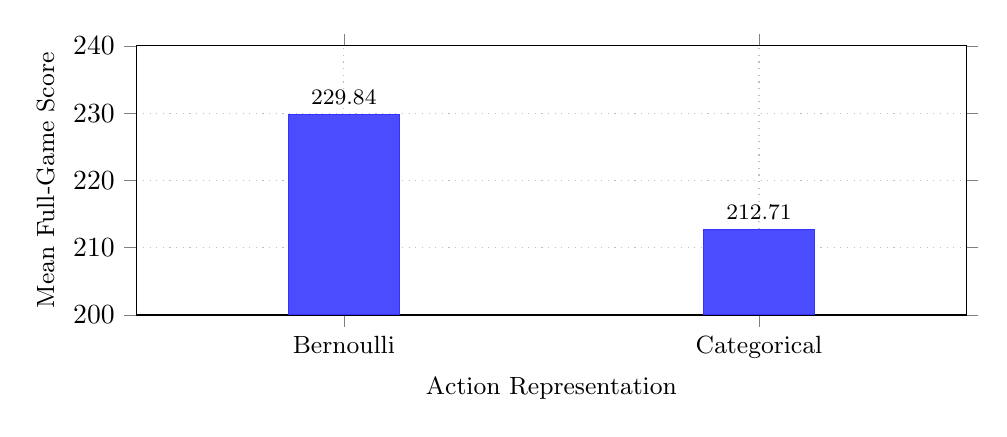
\begin{tikzpicture}
        \begin{axis}[
                ybar,
                width=\columnwidth,
                height=5cm,
                xlabel={Action Representation},
                ylabel={Mean Full-Game Score},
                symbolic x coords={Bernoulli, Categorical},
                xtick=data,
                xticklabel style={font=\small},
                ylabel style={font=\small},
                xlabel style={font=\small},
                bar width=40pt,
                ymin=200, ymax=240,
                grid=both,
                grid style={dotted},
                tick align=outside,
                nodes near coords,
                nodes near coords style={font=\footnotesize, anchor=south},
                enlarge x limits=0.5,
            ]

            \addplot[
                fill=blue!70!white,
                draw=blue!80,
                error bars/.cd,
                y dir=both,
                y explicit
            ] coordinates {
                    (Bernoulli, 229.84)
                    (Categorical, 212.71)
                };

        \end{axis}
    \end{tikzpicture}
    \caption{Performance comparison: Bernoulli vs Categorical action representation}
    \label{fig:bernoulli-vs-categorical}
\end{figure}

\begin{figure}[htb]
    \centering
    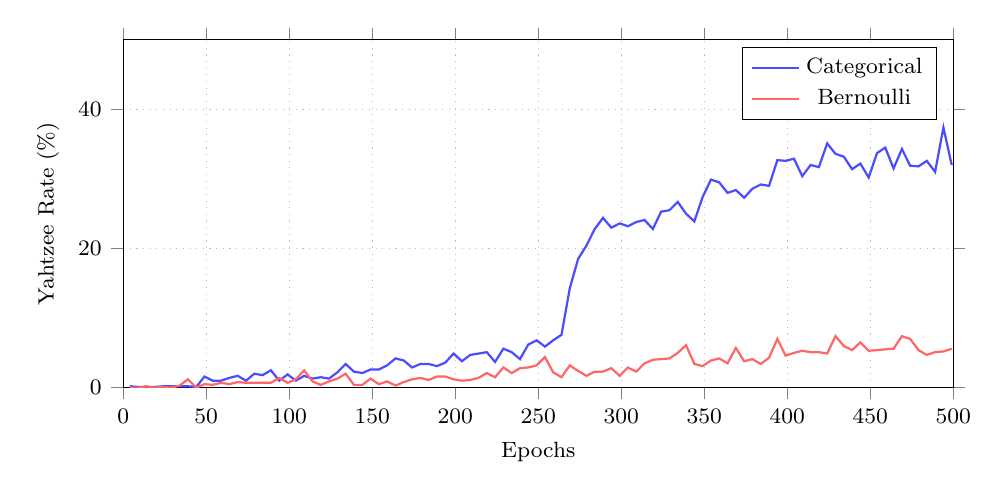
\begin{tikzpicture}
        \begin{axis}[
                width=\columnwidth,
                height=6cm,
                xlabel={Epochs},
                ylabel={Yahtzee Rate (\%)},
                xmin=0, xmax=500,
                ymin=0, ymax=50,
                grid=both,
                grid style={dotted},
                tick align=outside,
                tick label style={font=\footnotesize},
                label style={font=\footnotesize},
                legend style={at={(0.98,0.98)},anchor=north east,font=\footnotesize}
            ]

            % Categorical (glowing-sweep-1)
            \addplot[
                thick,
                blue!70!white
            ] coordinates {
                    (4, 0.2) (9, 0.1) (14, 0.1) (19, 0.1) (24, 0.2) (29, 0.2) (34, 0.2) (39, 0.2) (44, 0.1) (49, 1.6) (54, 1) (59, 1) (64, 1.4) (69, 1.7) (74, 1) (79, 2) (84, 1.8) (89, 2.5) (94, 1) (99, 1.9) (104, 1) (109, 1.7) (114, 1.3) (119, 1.5) (124, 1.3) (129, 2.2) (134, 3.4) (139, 2.3) (144, 2.1) (149, 2.6) (154, 2.6) (159, 3.2) (164, 4.2) (169, 3.9) (174, 2.9) (179, 3.4) (184, 3.4) (189, 3.1) (194, 3.6) (199, 4.9) (204, 3.8) (209, 4.7) (214, 4.9) (219, 5.1) (224, 3.7) (229, 5.6) (234, 5.1) (239, 4.1) (244, 6.2) (249, 6.8) (254, 5.9) (259, 6.8) (264, 7.6) (269, 14.3) (274, 18.5) (279, 20.4) (284, 22.8) (289, 24.4) (294, 23) (299, 23.6) (304, 23.2) (309, 23.8) (314, 24.1) (319, 22.8) (324, 25.3) (329, 25.5) (334, 26.7) (339, 25) (344, 23.9) (349, 27.4) (354, 29.9) (359, 29.5) (364, 28) (369, 28.4) (374, 27.3) (379, 28.6) (384, 29.2) (389, 29) (394, 32.7) (399, 32.6) (404, 32.9) (409, 30.4) (414, 32) (419, 31.7) (424, 35.1) (429, 33.6) (434, 33.2) (439, 31.4) (444, 32.2) (449, 30.2) (454, 33.7) (459, 34.5) (464, 31.5) (469, 34.3) (474, 31.9) (479, 31.8) (484, 32.6) (489, 31) (494, 37.4) (499, 32)
                };
            \addlegendentry{Categorical}

            % Bernoulli (helpful-sweep-2)
            \addplot[
                thick,
                red!60!white
            ] coordinates {
                    (4, 0) (9, 0) (14, 0.2) (19, 0) (24, 0.1) (29, 0) (34, 0.3) (39, 1.2) (44, 0) (49, 0.5) (54, 0.4) (59, 0.7) (64, 0.5) (69, 0.8) (74, 0.7) (79, 0.7) (84, 0.7) (89, 0.7) (94, 1.4) (99, 0.7) (104, 1.2) (109, 2.5) (114, 0.9) (119, 0.4) (124, 0.9) (129, 1.3) (134, 2) (139, 0.4) (144, 0.4) (149, 1.3) (154, 0.5) (159, 0.9) (164, 0.3) (169, 0.8) (174, 1.2) (179, 1.4) (184, 1.1) (189, 1.6) (194, 1.6) (199, 1.2) (204, 1) (209, 1.1) (214, 1.4) (219, 2.1) (224, 1.5) (229, 2.9) (234, 2.1) (239, 2.8) (244, 2.9) (249, 3.2) (254, 4.4) (259, 2.2) (264, 1.5) (269, 3.2) (274, 2.4) (279, 1.7) (284, 2.3) (289, 2.3) (294, 2.8) (299, 1.7) (304, 2.9) (309, 2.3) (314, 3.5) (319, 4) (324, 4.1) (329, 4.2) (334, 5) (339, 6.1) (344, 3.4) (349, 3.1) (354, 3.9) (359, 4.2) (364, 3.5) (369, 5.7) (374, 3.8) (379, 4.1) (384, 3.4) (389, 4.3) (394, 7) (399, 4.6) (404, 5) (409, 5.3) (414, 5.1) (419, 5.1) (424, 4.9) (429, 7.4) (434, 6) (439, 5.4) (444, 6.5) (449, 5.3) (454, 5.4) (459, 5.5) (464, 5.6) (469, 7.4) (474, 7) (479, 5.4) (484, 4.7) (489, 5.1) (494, 5.2) (499, 5.6)
                };
            \addlegendentry{Bernoulli}

        \end{axis}
    \end{tikzpicture}
    \caption{Learning Yahtzee with different action representations}
    \label{fig:action-yahtzee-learning}
\end{figure}

\subsubsection{Architectural Ablations}

We performed a simple grid search ablation to understand if our chosen architecture of 3 hidden layers of 600 units each was optimal.
Yahtzee is a fairly complex game, so we expected shorter, but wider networks to perform best. Note that each of these has a different number of total parameters,
so this is not a pure ablation of depth vs. width.

\begin{figure}[t]
    \centering
    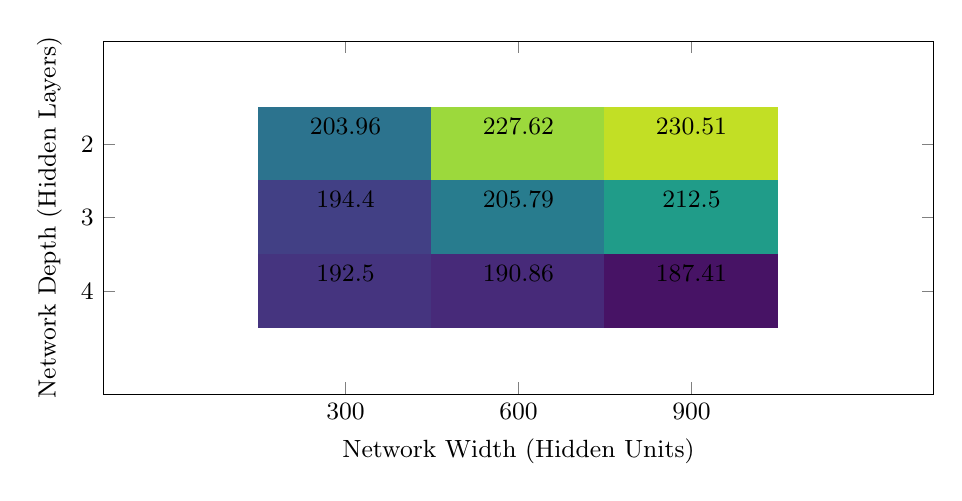
\begin{tikzpicture}
        \begin{axis}[
                width=\columnwidth,
                height=0.5\textwidth,
                xlabel={Network Width (Hidden Units)},
                ylabel={Network Depth (Hidden Layers)},
                colormap/viridis,
                xlabel style={font=\small},
                ylabel style={font=\small},
                title style={font=\small},
                xtick={1,2,3},
                xticklabels={300, 600, 900},
                ytick={1,2,3},
                yticklabels={2, 3, 4},
                xticklabel style={font=\small},
                yticklabel style={font=\small},
                enlargelimits=0.3,
                point meta min=185,
                point meta max=235,
                nodes near coords,
                nodes near coords style={font=\small, color=black},
                every node near coord/.append style={xshift=0pt, yshift=0pt},
            ]

            \addplot[
                matrix plot,
                mesh/cols=3,
                point meta=explicit
            ] table[meta=score] {
                    x y score
                    1 1 203.959
                    2 1 227.618
                    3 1 230.508
                    1 2 194.403
                    2 2 205.788
                    3 2 212.495
                    1 3 192.501
                    2 3 190.864
                    3 3 187.407
                };

        \end{axis}
    \end{tikzpicture}
    \caption{Network size ablation}
    \label{fig:architecture-heatmap}
\end{figure}


Based on \cite{bjorck-2022-high-variance}, we hypothesized that layer normalization \cite{ba-2016-layernorm} would improve training stability and performance
and used it in all of our main experiments. This was ablated to understand its true impact.


\begin{figure}[b]
    \centering
    % Panel (a): Learning curves
    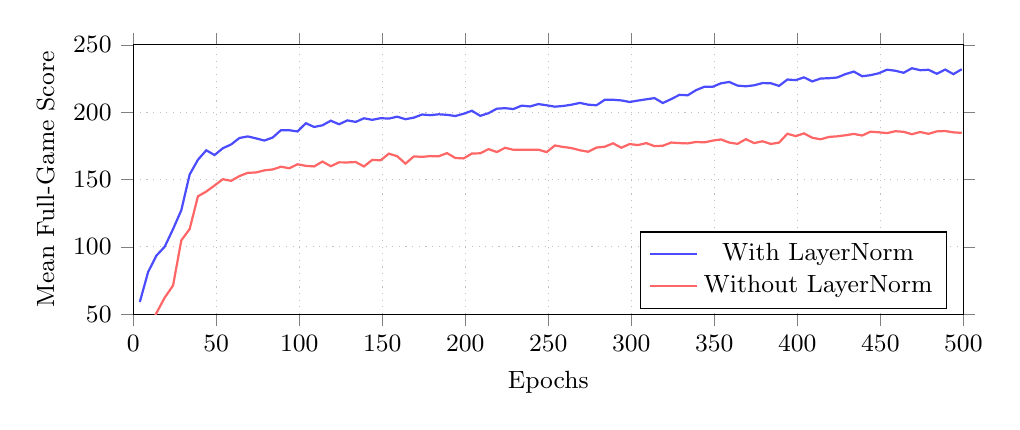
\begin{tikzpicture}
        \begin{axis}[
                width=\columnwidth,
                height=5cm,
                xlabel={Epochs},
                ylabel={Mean Full-Game Score},
                xmin=0, xmax=500,
                ymin=50, ymax=250,
                grid=both,
                grid style={dotted},
                tick align=outside,
                tick label style={font=\small},
                label style={font=\small},
                legend style={at={(0.98,0.02)},anchor=south east,font=\small}
            ]

            % With LayerNorm
            \addplot[
                thick,
                blue!70!white
            ] coordinates {
                    (4, 58.999000549316406)
                    (9, 81.2969970703125)
                    (14, 93.4739990234375)
                    (19, 100.08699798583984)
                    (24, 113.13899993896484)
                    (29, 127.22200012207031)
                    (34, 153.6699981689453)
                    (39, 164.68699645996094)
                    (44, 171.68299865722656)
                    (49, 168.16600036621094)
                    (54, 173.22300720214844)
                    (59, 176.0590057373047)
                    (64, 180.85299682617188)
                    (69, 182.00799560546875)
                    (74, 180.55999755859375)
                    (79, 178.93699645996094)
                    (84, 181.1750030517578)
                    (89, 186.63999938964844)
                    (94, 186.59500122070312)
                    (99, 185.69900512695312)
                    (104, 191.8249969482422)
                    (109, 189.031005859375)
                    (114, 190.26300048828125)
                    (119, 193.6840057373047)
                    (124, 191.0489959716797)
                    (129, 193.9250030517578)
                    (134, 192.79600524902344)
                    (139, 195.4770050048828)
                    (144, 194.33799743652344)
                    (149, 195.56100463867188)
                    (154, 195.2570037841797)
                    (159, 196.65899658203125)
                    (164, 194.81399536132812)
                    (169, 195.9459991455078)
                    (174, 198.28700256347656)
                    (179, 197.79800415039062)
                    (184, 198.44900512695312)
                    (189, 198.05599975585938)
                    (194, 197.17100524902344)
                    (199, 198.86900329589844)
                    (204, 201.08599853515625)
                    (209, 197.2989959716797)
                    (214, 199.28199768066406)
                    (219, 202.61000061035156)
                    (224, 202.98699951171875)
                    (229, 202.3699951171875)
                    (234, 204.88999938964844)
                    (239, 204.2729949951172)
                    (244, 206.05499267578125)
                    (249, 205.13600158691406)
                    (254, 204.1179962158203)
                    (259, 204.63800048828125)
                    (264, 205.5850067138672)
                    (269, 206.9149932861328)
                    (274, 205.61000061035156)
                    (279, 205.1510009765625)
                    (284, 209.2100067138672)
                    (289, 209.24899291992188)
                    (294, 208.76600646972656)
                    (299, 207.59800720214844)
                    (304, 208.64500427246094)
                    (309, 209.5970001220703)
                    (314, 210.49200439453125)
                    (319, 206.8280029296875)
                    (324, 209.73800659179688)
                    (329, 212.89599609375)
                    (334, 212.59100341796875)
                    (339, 216.38900756835938)
                    (344, 218.92100524902344)
                    (349, 218.89599609375)
                    (354, 221.48199462890625)
                    (359, 222.47000122070312)
                    (364, 219.7689971923828)
                    (369, 219.2570037841797)
                    (374, 220.00799560546875)
                    (379, 221.6439971923828)
                    (384, 221.52099609375)
                    (389, 219.5709991455078)
                    (394, 224.28399658203125)
                    (399, 223.83299255371094)
                    (404, 225.8699951171875)
                    (409, 222.88400268554688)
                    (414, 225.03399658203125)
                    (419, 225.25900268554688)
                    (424, 225.77099609375)
                    (429, 228.31100463867188)
                    (434, 230.20599365234375)
                    (439, 226.72799682617188)
                    (444, 227.50799560546875)
                    (449, 228.927001953125)
                    (454, 231.60400390625)
                    (459, 230.80599975585938)
                    (464, 229.29800415039062)
                    (469, 232.66400146484375)
                    (474, 231.2209930419922)
                    (479, 231.51499938964844)
                    (484, 228.57699584960938)
                    (489, 231.68899536132812)
                    (494, 228.27000427246094)
                    (499, 231.94000244140625)
                };
            \addlegendentry{With LayerNorm}

            % Without LayerNorm
            \addplot[
                thick,
                red!60!white
            ] coordinates {
                    (4, 47.832000732421875)
                    (9, 37.47999954223633)
                    (14, 50.750999450683594)
                    (19, 62.268001556396484)
                    (24, 71.1760025024414)
                    (29, 104.8290023803711)
                    (34, 113.16899871826172)
                    (39, 137.5019989013672)
                    (44, 141.0469970703125)
                    (49, 145.52999877929688)
                    (54, 150.21099853515625)
                    (59, 149.0229949951172)
                    (64, 152.5500030517578)
                    (69, 154.95700073242188)
                    (74, 155.23399353027344)
                    (79, 156.7899932861328)
                    (84, 157.4739990234375)
                    (89, 159.4810028076172)
                    (94, 158.35699462890625)
                    (99, 161.31500244140625)
                    (104, 160.13600158691406)
                    (109, 159.7100067138672)
                    (114, 163.3209991455078)
                    (119, 159.88099670410156)
                    (124, 162.7480010986328)
                    (129, 162.6790008544922)
                    (134, 162.98800659179688)
                    (139, 159.69500732421875)
                    (144, 164.60299682617188)
                    (149, 164.24899291992188)
                    (154, 169.21499633789062)
                    (159, 167.28399658203125)
                    (164, 161.77699279785156)
                    (169, 167.17599487304688)
                    (174, 166.82699584960938)
                    (179, 167.375)
                    (184, 167.2310028076172)
                    (189, 169.63099670410156)
                    (194, 165.99200439453125)
                    (199, 165.66900634765625)
                    (204, 169.30499267578125)
                    (209, 169.46499633789062)
                    (214, 172.58399963378906)
                    (219, 170.41700744628906)
                    (224, 173.5590057373047)
                    (229, 172.0659942626953)
                    (234, 172.10000610351562)
                    (239, 172.05799865722656)
                    (244, 172.17100524902344)
                    (249, 170.36599731445312)
                    (254, 175.3040008544922)
                    (259, 174.16299438476562)
                    (264, 173.3520050048828)
                    (269, 171.72000122070312)
                    (274, 170.62600708007812)
                    (279, 173.73599243164062)
                    (284, 174.37399291992188)
                    (289, 176.88299560546875)
                    (294, 173.61700439453125)
                    (299, 176.33700561523438)
                    (304, 175.59100341796875)
                    (309, 177.0229949951172)
                    (314, 174.78599548339844)
                    (319, 175.08299255371094)
                    (324, 177.45799255371094)
                    (329, 177.052001953125)
                    (334, 176.81700134277344)
                    (339, 177.90199279785156)
                    (344, 177.58900451660156)
                    (349, 178.89500427246094)
                    (354, 179.7469940185547)
                    (359, 177.42599487304688)
                    (364, 176.5)
                    (369, 179.9949951171875)
                    (374, 177.03599548339844)
                    (379, 178.40899658203125)
                    (384, 176.42300415039062)
                    (389, 177.4239959716797)
                    (394, 184.01199340820312)
                    (399, 182.24400329589844)
                    (404, 184.26499938964844)
                    (409, 181.0019989013672)
                    (414, 179.8679962158203)
                    (419, 181.6280059814453)
                    (424, 182.0749969482422)
                    (429, 182.88400268554688)
                    (434, 183.86900329589844)
                    (439, 182.68499755859375)
                    (444, 185.50999450683594)
                    (449, 185.08799743652344)
                    (454, 184.48300170898438)
                    (459, 185.86500549316406)
                    (464, 185.43499755859375)
                    (469, 183.65699768066406)
                    (474, 185.2830047607422)
                    (479, 183.93699645996094)
                    (484, 185.7480010986328)
                    (489, 186.0290069580078)
                    (494, 185.02999877929688)
                    (499, 184.6479949951172)
                };
            \addlegendentry{Without LayerNorm}

        \end{axis}
    \end{tikzpicture}
    \caption{Learning curves with and without LayerNorm}
    \label{fig:layernorm-learning}
\end{figure}

Lastly, we used Swish activation functions in our network for all of our main experiments, as it had been reported to work well in RL settings \cite{elfwing2017sigmoidweightedlinearunitsneural}.
We ablated this to ReLU to understand its true impact.

\begin{figure}[htb]
    \centering
    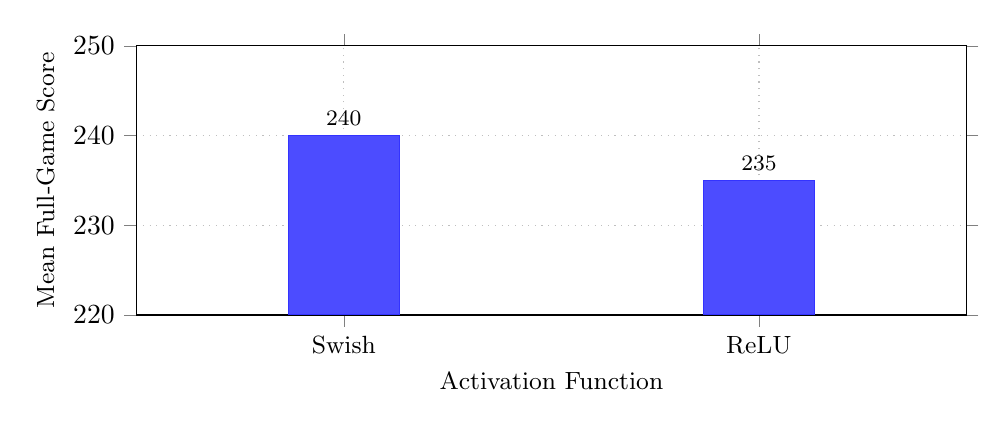
\begin{tikzpicture}
        \begin{axis}[
                ybar,
                width=\columnwidth,
                height=5cm,
                xlabel={Activation Function},
                ylabel={Mean Full-Game Score},
                symbolic x coords={Swish, ReLU},
                xtick=data,
                xticklabel style={font=\small},
                ylabel style={font=\small},
                xlabel style={font=\small},
                bar width=40pt,
                ymin=220, ymax=250,
                grid=both,
                grid style={dotted},
                tick align=outside,
                nodes near coords,
                nodes near coords style={font=\footnotesize, anchor=south},
                enlarge x limits=0.5,
            ]

            \addplot[
                fill=blue!70!white,
                draw=blue!80,
                error bars/.cd,
                y dir=both,
                y explicit
            ] coordinates {
                    (Swish, 240)
                    (ReLU, 235)
                };

        \end{axis}
    \end{tikzpicture}
    \caption{Performance comparison: Swish vs ReLU activation (placeholder data)}
    \label{fig:silu-vs-relu}
\end{figure}


\subsubsection{Credit Assignment: TD(0) vs GAE}

Later in this research, we noticed the main issue with our network was that it was struggling to earn the bonus, learning it very slowly.
We first hypothesized that this was due to high variance in REINFORCE, so we switched to A2C with TD(0) targets. However, the issue
persisted. We then hypothesized that the TD(0) targets were not providing sufficient credit assignment for the long-term bonus reward,
so we switched to GAE with various $\lambda$ values to understand if this would help.

Unfortunately, we found that GAE did not improve performance over TD(0), and values that were too high ($\lambda \geq 0.8$)
significantly degraded performance.

\begin{figure}[htb]
    \centering
    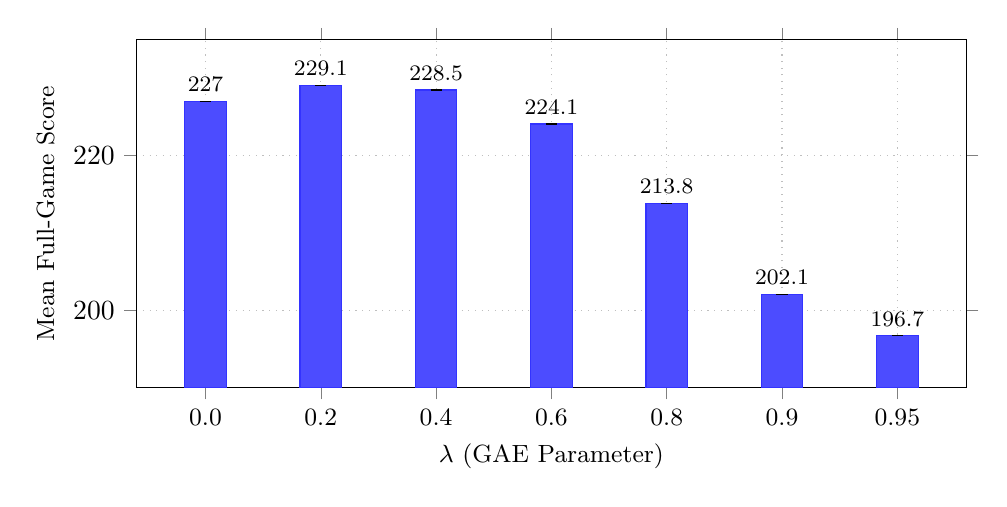
\begin{tikzpicture}
        \begin{axis}[
                ybar,
                width=\columnwidth,
                height=6cm,
                xlabel={$\lambda$ (GAE Parameter)},
                ylabel={Mean Full-Game Score},
                symbolic x coords={0.0, 0.2, 0.4, 0.6, 0.8, 0.9, 0.95},
                xtick=data,
                xticklabel style={font=\small},
                ylabel style={font=\small},
                xlabel style={font=\small},
                bar width=15pt,
                ymin=190, ymax=235,
                grid=both,
                grid style={dotted},
                tick align=outside,
                nodes near coords,
                nodes near coords style={font=\footnotesize, anchor=south},
            ]

            \addplot[
                fill=blue!70!white,
                draw=blue!80!white,
                error bars/.cd,
                y dir=both,
                y explicit
            ] coordinates {
                    (0.0, 227.0) +- (0, 0)
                    (0.2, 229.1) +- (0, 0)
                    (0.4, 228.5) +- (0, 0)
                    (0.6, 224.1) +- (0, 0)
                    (0.8, 213.8) +- (0, 0)
                    (0.9, 202.1) +- (0, 0)
                    (0.95, 196.7) +- (0, 0)
                };

        \end{axis}
    \end{tikzpicture}
    \caption{Final performance by GAE lambda}
    \label{fig:gae-lambda-performance}
\end{figure}
\begin{figure}[H]
    \centering
    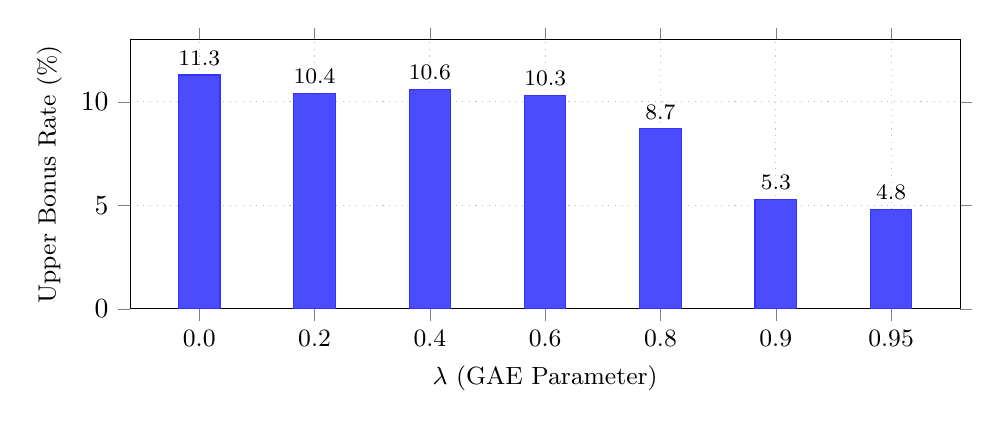
\begin{tikzpicture}
        \begin{axis}[
                ybar,
                width=\columnwidth,
                height=5cm,
                xlabel={$\lambda$ (GAE Parameter)},
                ylabel={Upper Bonus Rate (\%)},
                symbolic x coords={0.0, 0.2, 0.4, 0.6, 0.8, 0.9, 0.95},
                xtick=data,
                xticklabel style={font=\small},
                ylabel style={font=\small},
                xlabel style={font=\small},
                bar width=15pt,
                ymin=0, ymax=13,
                grid=both,
                grid style={dotted},
                tick align=outside,
                nodes near coords,
                nodes near coords style={font=\footnotesize, anchor=south},
            ]

            \addplot[
                fill=blue!70!white,
                draw=blue!80!white,
                error bars/.cd,
                y dir=both,
                y explicit
            ] coordinates {
                    (0.0, 11.3)
                    (0.2, 10.4)
                    (0.4, 10.6)
                    (0.6, 10.3)
                    (0.8, 8.7)
                    (0.9, 5.3)
                    (0.95, 4.8)
                };

        \end{axis}
    \end{tikzpicture}
    \caption{Upper bonus achievement by GAE lambda}
    \label{fig:gae-lambda-bonus}
\end{figure}


\subsubsection{Entropy Sensitivity}
During experimentation, we noticed that the entropy regularization coefficients had a significant impact on training stability and final performance.
With no regularization, the policy quickly converges to a deterministic policy that fails to explore sufficiently.
With too much regularization, the policy would not perform well enough to quickly learn strategies for earning Yahtzee's and the bonus.
To better understand this sensitivity, we trained models under three different entropy regimes: Low Entropy, Baseline, and High Entropy.

\begin{table}[H]
    \centering
    \small
    \caption{Entropy regime definitions}
    \label{tab:entropy-regime-definitions}
    \begin{tabular}{lcccc}
        \hline
        \textbf{Regime} & $\beta_{\mathrm{roll}}$ & $\beta_{\mathrm{score}}$ & Hold / Anneal \\
        \hline
        None            & 0.0                     & 0.0                      & 0 / 0         \\
        Low             & 0.05 $\rightarrow$ 0.01 & 0.01 $\rightarrow$ 0.005 & 0.2 / 0.4     \\
        Baseline        & 0.1 $\rightarrow$ 0.02  & 0.03 $\rightarrow$ 0.01  & 0.3 / 0.6     \\
        High            & 0.2 $\rightarrow$ 0.04  & 0.06 $\rightarrow$ 0.02  & 0.35 / 0.65   \\
        \hline
    \end{tabular}
\end{table}


\begin{figure}[H]
    \centering
    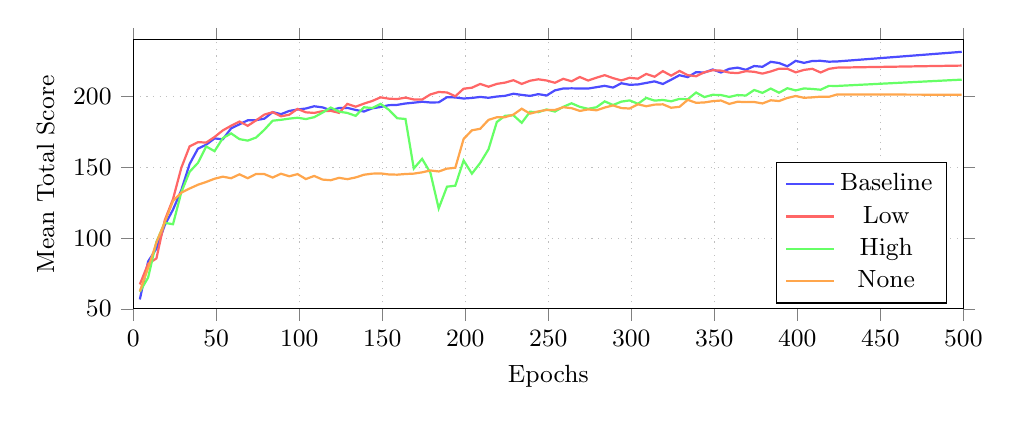
\begin{tikzpicture}
        \begin{axis}[
                width=\columnwidth,
                height=5cm,
                xlabel={Epochs},
                ylabel={Mean Total Score},
                xmin=0, xmax=500,
                ymin=50, ymax=240,
                grid=both,
                grid style={dotted},
                tick align=outside,
                tick label style={font=\small},
                label style={font=\small},
                legend style={at={(0.98,0.02)},anchor=south east,font=\small}
            ]

            % Baseline
            \addplot[
                thick,
                blue!70!white
            ] coordinates {
                    (4, 56.721)
                    (9, 83.499)
                    (14, 92.566)
                    (19, 109.083)
                    (24, 120.138)
                    (29, 133.889)
                    (34, 152.331)
                    (39, 163.122)
                    (44, 165.951)
                    (49, 170.356)
                    (54, 169.733)
                    (59, 177.495)
                    (64, 180.302)
                    (69, 183.169)
                    (74, 183.267)
                    (79, 184.294)
                    (84, 188.940)
                    (89, 187.466)
                    (94, 189.754)
                    (99, 190.778)
                    (104, 191.467)
                    (109, 193.057)
                    (114, 192.273)
                    (119, 190.236)
                    (124, 191.819)
                    (129, 191.914)
                    (134, 190.466)
                    (139, 189.351)
                    (144, 191.613)
                    (149, 192.538)
                    (154, 193.830)
                    (159, 194.032)
                    (164, 195.014)
                    (169, 195.584)
                    (174, 196.254)
                    (179, 195.733)
                    (184, 195.822)
                    (189, 199.468)
                    (194, 199.287)
                    (199, 198.519)
                    (204, 198.928)
                    (209, 199.650)
                    (214, 199.048)
                    (219, 199.925)
                    (224, 200.425)
                    (229, 201.890)
                    (234, 201.076)
                    (239, 200.381)
                    (244, 201.611)
                    (249, 200.665)
                    (254, 204.277)
                    (259, 205.592)
                    (264, 205.708)
                    (269, 205.607)
                    (274, 205.556)
                    (279, 206.528)
                    (284, 207.483)
                    (289, 206.256)
                    (294, 209.300)
                    (299, 208.201)
                    (304, 208.444)
                    (309, 209.533)
                    (314, 210.622)
                    (319, 208.792)
                    (324, 211.803)
                    (329, 214.965)
                    (334, 213.620)
                    (339, 217.120)
                    (344, 216.871)
                    (349, 219.041)
                    (354, 216.889)
                    (359, 219.496)
                    (364, 220.331)
                    (369, 218.815)
                    (374, 221.462)
                    (379, 220.925)
                    (384, 224.419)
                    (389, 223.578)
                    (394, 221.263)
                    (399, 225.132)
                    (404, 223.684)
                    (409, 225.015)
                    (414, 225.142)
                    (419, 224.519)
                    (424, 224.686)
                    (499, 231.481)
                };
            \addlegendentry{Baseline}

            % Low Entropy
            \addplot[
                thick,
                red!60!white
            ] coordinates {
                    (4, 67.316)
                    (9, 81.865)
                    (14, 85.635)
                    (19, 112.538)
                    (24, 127.582)
                    (29, 149.650)
                    (34, 164.766)
                    (39, 167.716)
                    (44, 167.439)
                    (49, 171.358)
                    (54, 176.024)
                    (59, 179.318)
                    (64, 182.247)
                    (69, 179.291)
                    (74, 183.071)
                    (79, 187.177)
                    (84, 188.875)
                    (89, 185.954)
                    (94, 187.118)
                    (99, 191.192)
                    (104, 188.778)
                    (109, 188.363)
                    (114, 189.562)
                    (119, 189.824)
                    (124, 188.413)
                    (129, 194.738)
                    (134, 192.748)
                    (139, 194.920)
                    (144, 196.817)
                    (149, 199.363)
                    (154, 198.408)
                    (159, 198.149)
                    (164, 199.157)
                    (169, 197.876)
                    (174, 197.797)
                    (179, 201.411)
                    (184, 203.139)
                    (189, 202.801)
                    (194, 200.133)
                    (199, 205.445)
                    (204, 206.162)
                    (209, 208.809)
                    (214, 206.832)
                    (219, 208.851)
                    (224, 209.758)
                    (229, 211.448)
                    (234, 208.829)
                    (239, 211.076)
                    (244, 212.093)
                    (249, 211.245)
                    (254, 209.635)
                    (259, 212.433)
                    (264, 210.702)
                    (269, 213.698)
                    (274, 211.210)
                    (279, 213.229)
                    (284, 215.008)
                    (289, 212.922)
                    (294, 211.288)
                    (299, 213.162)
                    (304, 212.530)
                    (309, 215.885)
                    (314, 213.907)
                    (319, 217.841)
                    (324, 214.658)
                    (329, 217.983)
                    (334, 215.025)
                    (339, 214.257)
                    (344, 217.058)
                    (349, 218.474)
                    (354, 218.214)
                    (359, 216.834)
                    (364, 216.456)
                    (369, 217.825)
                    (374, 217.379)
                    (379, 216.108)
                    (384, 217.626)
                    (389, 219.591)
                    (394, 219.520)
                    (399, 216.999)
                    (404, 218.721)
                    (409, 219.504)
                    (414, 216.887)
                    (419, 219.453)
                    (424, 220.336)
                    (499, 221.776)
                };
            \addlegendentry{Low}

            % High Entropy
            \addplot[
                thick,
                green!60!white
            ] coordinates {
                    (4, 62.074)
                    (9, 72.131)
                    (14, 97.401)
                    (19, 110.767)
                    (24, 109.796)
                    (29, 132.415)
                    (34, 146.830)
                    (39, 153.090)
                    (44, 164.659)
                    (49, 161.340)
                    (54, 170.565)
                    (59, 173.896)
                    (64, 169.861)
                    (69, 168.814)
                    (74, 170.970)
                    (79, 176.432)
                    (84, 182.864)
                    (89, 183.488)
                    (94, 184.339)
                    (99, 184.967)
                    (104, 184.020)
                    (109, 185.339)
                    (114, 188.564)
                    (119, 192.182)
                    (124, 189.262)
                    (129, 188.346)
                    (134, 186.276)
                    (139, 192.365)
                    (144, 191.805)
                    (149, 194.757)
                    (154, 190.556)
                    (159, 184.599)
                    (164, 184.076)
                    (169, 149.129)
                    (174, 155.934)
                    (179, 146.127)
                    (184, 120.973)
                    (189, 136.300)
                    (194, 136.990)
                    (199, 154.795)
                    (204, 145.498)
                    (209, 153.057)
                    (214, 162.687)
                    (219, 181.936)
                    (224, 186.364)
                    (229, 186.678)
                    (234, 181.374)
                    (239, 189.171)
                    (244, 188.890)
                    (249, 190.806)
                    (254, 189.314)
                    (259, 192.650)
                    (264, 195.163)
                    (269, 192.639)
                    (274, 191.254)
                    (279, 192.363)
                    (284, 196.502)
                    (289, 193.930)
                    (294, 196.324)
                    (299, 197.187)
                    (304, 194.800)
                    (309, 198.967)
                    (314, 197.062)
                    (319, 197.491)
                    (324, 196.540)
                    (329, 198.271)
                    (334, 197.979)
                    (339, 202.760)
                    (344, 199.547)
                    (349, 201.154)
                    (354, 200.970)
                    (359, 199.649)
                    (364, 200.976)
                    (369, 200.644)
                    (374, 204.518)
                    (379, 202.521)
                    (384, 205.570)
                    (389, 202.635)
                    (394, 205.782)
                    (399, 204.241)
                    (404, 205.643)
                    (409, 205.267)
                    (414, 204.736)
                    (419, 207.457)
                    (424, 207.400)
                    (499, 211.854)
                };
            \addlegendentry{High}

            % No Entropy
            \addplot[
                thick,
                orange!70!white
            ] coordinates {
                    (4, 62.409)
                    (9, 78.939)
                    (14, 96.791)
                    (19, 111.213)
                    (24, 126.241)
                    (29, 132.096)
                    (34, 134.982)
                    (39, 137.650)
                    (44, 139.643)
                    (49, 141.896)
                    (54, 143.355)
                    (59, 142.258)
                    (64, 145.008)
                    (69, 142.270)
                    (74, 145.274)
                    (79, 145.185)
                    (84, 142.736)
                    (89, 145.457)
                    (94, 143.632)
                    (99, 145.161)
                    (104, 141.688)
                    (109, 143.866)
                    (114, 141.320)
                    (119, 140.865)
                    (124, 142.554)
                    (129, 141.586)
                    (134, 142.822)
                    (139, 144.715)
                    (144, 145.495)
                    (149, 145.671)
                    (154, 144.926)
                    (159, 144.775)
                    (164, 145.239)
                    (169, 145.509)
                    (174, 146.420)
                    (179, 147.734)
                    (184, 147.036)
                    (189, 149.029)
                    (194, 149.642)
                    (199, 169.970)
                    (204, 176.076)
                    (209, 177.166)
                    (214, 183.453)
                    (219, 185.276)
                    (224, 185.376)
                    (229, 187.186)
                    (234, 191.325)
                    (239, 187.843)
                    (244, 189.419)
                    (249, 190.464)
                    (254, 190.438)
                    (259, 192.393)
                    (264, 191.715)
                    (269, 189.756)
                    (274, 190.851)
                    (279, 190.210)
                    (284, 192.179)
                    (289, 193.659)
                    (294, 191.778)
                    (299, 191.459)
                    (304, 194.454)
                    (309, 193.072)
                    (314, 194.198)
                    (319, 194.426)
                    (324, 192.014)
                    (329, 192.652)
                    (334, 197.587)
                    (339, 195.511)
                    (344, 195.743)
                    (349, 196.670)
                    (354, 197.103)
                    (359, 194.708)
                    (364, 196.261)
                    (369, 195.988)
                    (374, 196.064)
                    (379, 195.044)
                    (384, 197.279)
                    (389, 196.747)
                    (394, 198.931)
                    (399, 200.284)
                    (404, 199.041)
                    (409, 199.337)
                    (414, 199.848)
                    (419, 199.716)
                    (424, 201.402)
                    (499, 201.193)
                };
            \addlegendentry{None}

        \end{axis}
    \end{tikzpicture}
    \caption{Mean total score across training epochs for different entropy regimes}
    \label{fig:entropy-rolling}
\end{figure}

\begin{figure}[H]
    \centering
    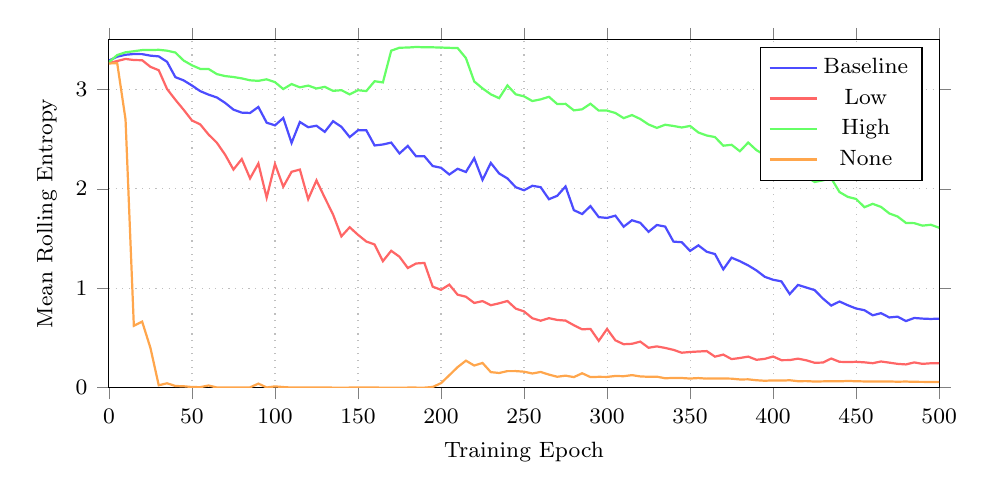
\begin{tikzpicture}
        \begin{axis}[
                width=\columnwidth,
                height=6cm,
                xlabel={Training Epoch},
                ylabel={Mean Rolling Entropy},
                xmin=0, xmax=500,
                ymin=0, ymax=3.5,
                grid=both,
                grid style={dotted},
                tick align=outside,
                tick label style={font=\footnotesize},
                label style={font=\footnotesize},
                legend style={at={(0.98,0.98)},anchor=north east,font=\footnotesize}
            ]

            % Baseline (misty-night-795)
            \addplot[
                thick,
                blue!70!white
            ] coordinates {
                    (0, 3.2908)
                    (5, 3.3296)
                    (10, 3.3492)
                    (15, 3.3566)
                    (20, 3.3553)
                    (25, 3.3401)
                    (30, 3.3325)
                    (35, 3.2780)
                    (40, 3.1242)
                    (45, 3.0912)
                    (50, 3.0397)
                    (55, 2.9831)
                    (60, 2.9479)
                    (65, 2.9193)
                    (70, 2.8649)
                    (75, 2.7969)
                    (80, 2.7669)
                    (85, 2.7637)
                    (90, 2.8238)
                    (95, 2.6660)
                    (100, 2.6386)
                    (105, 2.7133)
                    (110, 2.4628)
                    (115, 2.6727)
                    (120, 2.6203)
                    (125, 2.6350)
                    (130, 2.5735)
                    (135, 2.6806)
                    (140, 2.6240)
                    (145, 2.5208)
                    (150, 2.5894)
                    (155, 2.5893)
                    (160, 2.4364)
                    (165, 2.4463)
                    (170, 2.4654)
                    (175, 2.3562)
                    (180, 2.4321)
                    (185, 2.3272)
                    (190, 2.3278)
                    (195, 2.2294)
                    (200, 2.2124)
                    (205, 2.1443)
                    (210, 2.2021)
                    (215, 2.1695)
                    (220, 2.3079)
                    (225, 2.0904)
                    (230, 2.2608)
                    (235, 2.1548)
                    (240, 2.1048)
                    (245, 2.0166)
                    (250, 1.9859)
                    (255, 2.0307)
                    (260, 2.0171)
                    (265, 1.8959)
                    (270, 1.9302)
                    (275, 2.0242)
                    (280, 1.7859)
                    (285, 1.7467)
                    (290, 1.8264)
                    (295, 1.7154)
                    (300, 1.7075)
                    (305, 1.7302)
                    (310, 1.6191)
                    (315, 1.6839)
                    (320, 1.6584)
                    (325, 1.5681)
                    (330, 1.6364)
                    (335, 1.6205)
                    (340, 1.4692)
                    (345, 1.4632)
                    (350, 1.3758)
                    (355, 1.4317)
                    (360, 1.3676)
                    (365, 1.3439)
                    (370, 1.1899)
                    (375, 1.3074)
                    (380, 1.2722)
                    (385, 1.2299)
                    (390, 1.1789)
                    (395, 1.1150)
                    (400, 1.0855)
                    (405, 1.0692)
                    (410, 0.9417)
                    (415, 1.0334)
                    (420, 1.0074)
                    (425, 0.9816)
                    (430, 0.8966)
                    (435, 0.8259)
                    (440, 0.8667)
                    (445, 0.8290)
                    (450, 0.7960)
                    (455, 0.7791)
                    (460, 0.7280)
                    (465, 0.7494)
                    (470, 0.7062)
                    (475, 0.7141)
                    (480, 0.6699)
                    (485, 0.7010)
                    (490, 0.6947)
                    (495, 0.6912)
                    (500, 0.6943)
                };
            \addlegendentry{Baseline}

            % Low Entropy (earthy-moon-792)
            \addplot[
                thick,
                red!60!white
            ] coordinates {
                    (0, 3.2655)
                    (5, 3.2863)
                    (10, 3.3070)
                    (15, 3.2961)
                    (20, 3.2941)
                    (25, 3.2276)
                    (30, 3.1934)
                    (35, 3.0048)
                    (40, 2.8967)
                    (45, 2.7956)
                    (50, 2.6885)
                    (55, 2.6482)
                    (60, 2.5468)
                    (65, 2.4641)
                    (70, 2.3430)
                    (75, 2.1942)
                    (80, 2.2997)
                    (85, 2.1055)
                    (90, 2.2552)
                    (95, 1.9117)
                    (100, 2.2503)
                    (105, 2.0217)
                    (110, 2.1716)
                    (115, 2.1942)
                    (120, 1.8960)
                    (125, 2.0852)
                    (130, 1.9105)
                    (135, 1.7414)
                    (140, 1.5220)
                    (145, 1.6138)
                    (150, 1.5378)
                    (155, 1.4703)
                    (160, 1.4405)
                    (165, 1.2724)
                    (170, 1.3770)
                    (175, 1.3168)
                    (180, 1.2036)
                    (185, 1.2491)
                    (190, 1.2547)
                    (195, 1.0158)
                    (200, 0.9845)
                    (205, 1.0364)
                    (210, 0.9353)
                    (215, 0.9148)
                    (220, 0.8521)
                    (225, 0.8705)
                    (230, 0.8293)
                    (235, 0.8487)
                    (240, 0.8718)
                    (245, 0.7953)
                    (250, 0.7670)
                    (255, 0.6983)
                    (260, 0.6734)
                    (265, 0.6992)
                    (270, 0.6811)
                    (275, 0.6747)
                    (280, 0.6280)
                    (285, 0.5868)
                    (290, 0.5911)
                    (295, 0.4708)
                    (300, 0.5903)
                    (305, 0.4762)
                    (310, 0.4370)
                    (315, 0.4412)
                    (320, 0.4631)
                    (325, 0.4014)
                    (330, 0.4151)
                    (335, 0.3997)
                    (340, 0.3801)
                    (345, 0.3515)
                    (350, 0.3589)
                    (355, 0.3636)
                    (360, 0.3678)
                    (365, 0.3118)
                    (370, 0.3324)
                    (375, 0.2873)
                    (380, 0.2982)
                    (385, 0.3124)
                    (390, 0.2803)
                    (395, 0.2898)
                    (400, 0.3133)
                    (405, 0.2766)
                    (410, 0.2774)
                    (415, 0.2918)
                    (420, 0.2752)
                    (425, 0.2504)
                    (430, 0.2525)
                    (435, 0.2930)
                    (440, 0.2599)
                    (445, 0.2578)
                    (450, 0.2599)
                    (455, 0.2546)
                    (460, 0.2461)
                    (465, 0.2632)
                    (470, 0.2515)
                    (475, 0.2393)
                    (480, 0.2336)
                    (485, 0.2539)
                    (490, 0.2393)
                    (495, 0.2453)
                    (500, 0.2450)
                };
            \addlegendentry{Low}

            % High Entropy (dandy-voice-791)
            \addplot[
                thick,
                green!60!white
            ] coordinates {
                    (0, 3.2742)
                    (5, 3.3464)
                    (10, 3.3738)
                    (15, 3.3845)
                    (20, 3.3961)
                    (25, 3.3962)
                    (30, 3.3989)
                    (35, 3.3902)
                    (40, 3.3715)
                    (45, 3.2907)
                    (50, 3.2432)
                    (55, 3.2067)
                    (60, 3.2060)
                    (65, 3.1546)
                    (70, 3.1344)
                    (75, 3.1252)
                    (80, 3.1113)
                    (85, 3.0920)
                    (90, 3.0865)
                    (95, 3.1021)
                    (100, 3.0734)
                    (105, 3.0042)
                    (110, 3.0544)
                    (115, 3.0213)
                    (120, 3.0388)
                    (125, 3.0098)
                    (130, 3.0262)
                    (135, 2.9856)
                    (140, 2.9928)
                    (145, 2.9504)
                    (150, 2.9923)
                    (155, 2.9838)
                    (160, 3.0827)
                    (165, 3.0710)
                    (170, 3.3900)
                    (175, 3.4199)
                    (180, 3.4216)
                    (185, 3.4272)
                    (190, 3.4245)
                    (195, 3.4238)
                    (200, 3.4218)
                    (205, 3.4186)
                    (210, 3.4167)
                    (215, 3.3156)
                    (220, 3.0805)
                    (225, 3.0107)
                    (230, 2.9509)
                    (235, 2.9123)
                    (240, 3.0404)
                    (245, 2.9510)
                    (250, 2.9306)
                    (255, 2.8835)
                    (260, 2.9002)
                    (265, 2.9262)
                    (270, 2.8533)
                    (275, 2.8552)
                    (280, 2.7896)
                    (285, 2.8003)
                    (290, 2.8562)
                    (295, 2.7872)
                    (300, 2.7873)
                    (305, 2.7633)
                    (310, 2.7113)
                    (315, 2.7423)
                    (320, 2.7031)
                    (325, 2.6478)
                    (330, 2.6134)
                    (335, 2.6450)
                    (340, 2.6326)
                    (345, 2.6175)
                    (350, 2.6329)
                    (355, 2.5670)
                    (360, 2.5368)
                    (365, 2.5210)
                    (370, 2.4343)
                    (375, 2.4432)
                    (380, 2.3785)
                    (385, 2.4660)
                    (390, 2.3891)
                    (395, 2.3403)
                    (400, 2.2852)
                    (405, 2.2011)
                    (410, 2.2101)
                    (415, 2.1963)
                    (420, 2.1209)
                    (425, 2.0693)
                    (430, 2.0855)
                    (435, 2.1062)
                    (440, 1.9678)
                    (445, 1.9190)
                    (450, 1.8982)
                    (455, 1.8153)
                    (460, 1.8493)
                    (465, 1.8182)
                    (470, 1.7526)
                    (475, 1.7216)
                    (480, 1.6574)
                    (485, 1.6551)
                    (490, 1.6298)
                    (495, 1.6389)
                    (500, 1.6088)
                };
            \addlegendentry{High}

            % No Entropy (peach-smoke-794)
            \addplot[
                thick,
                orange!70!white
            ] coordinates {
                    (0, 3.2616)
                    (5, 3.2639)
                    (10, 2.6988)
                    (15, 0.6226)
                    (20, 0.6647)
                    (25, 0.3996)
                    (30, 0.0239)
                    (35, 0.0440)
                    (40, 0.0167)
                    (45, 0.0139)
                    (50, 0.0064)
                    (55, 0.0050)
                    (60, 0.0217)
                    (65, 0.0017)
                    (70, 0.0012)
                    (75, 0.0017)
                    (80, 0.0020)
                    (85, 0.0028)
                    (90, 0.0405)
                    (95, 0.0018)
                    (100, 0.0128)
                    (105, 0.0059)
                    (110, 0.0010)
                    (115, 0.0007)
                    (120, 0.0021)
                    (125, 0.0018)
                    (130, 0.0010)
                    (135, 0.0004)
                    (140, 0.0004)
                    (145, 0.0005)
                    (150, 0.0005)
                    (155, 0.0005)
                    (160, 0.0007)
                    (165, 0.0003)
                    (170, 0.0003)
                    (175, 0.0003)
                    (180, 0.0005)
                    (185, 0.0005)
                    (190, 0.0001)
                    (195, 0.0069)
                    (200, 0.0453)
                    (205, 0.1250)
                    (210, 0.2065)
                    (215, 0.2715)
                    (220, 0.2226)
                    (225, 0.2485)
                    (230, 0.1563)
                    (235, 0.1476)
                    (240, 0.1664)
                    (245, 0.1665)
                    (250, 0.1607)
                    (255, 0.1425)
                    (260, 0.1580)
                    (265, 0.1312)
                    (270, 0.1096)
                    (275, 0.1207)
                    (280, 0.1061)
                    (285, 0.1447)
                    (290, 0.1065)
                    (295, 0.1089)
                    (300, 0.1081)
                    (305, 0.1174)
                    (310, 0.1152)
                    (315, 0.1260)
                    (320, 0.1131)
                    (325, 0.1091)
                    (330, 0.1102)
                    (335, 0.0946)
                    (340, 0.0975)
                    (345, 0.0968)
                    (350, 0.0918)
                    (355, 0.0964)
                    (360, 0.0909)
                    (365, 0.0929)
                    (370, 0.0920)
                    (375, 0.0906)
                    (380, 0.0823)
                    (385, 0.0837)
                    (390, 0.0745)
                    (395, 0.0694)
                    (400, 0.0730)
                    (405, 0.0709)
                    (410, 0.0744)
                    (415, 0.0650)
                    (420, 0.0658)
                    (425, 0.0616)
                    (430, 0.0633)
                    (435, 0.0646)
                    (440, 0.0635)
                    (445, 0.0673)
                    (450, 0.0644)
                    (455, 0.0627)
                    (460, 0.0613)
                    (465, 0.0625)
                    (470, 0.0619)
                    (475, 0.0598)
                    (480, 0.0614)
                    (485, 0.0585)
                    (490, 0.0582)
                    (495, 0.0569)
                    (500, 0.0559)
                };
            \addlegendentry{None}

        \end{axis}
    \end{tikzpicture}
    \caption{Mean rolling entropy across training epochs for different entropy regularization settings}
    \label{fig:entropy-rolling}
\end{figure}
% Data sources:
% Baseline: misty-night-795 - train/entropy_roll
% Low Entropy: earthy-moon-792 - train/entropy_roll
% High Entropy: dandy-voice-791 - train/entropy_roll
% No Entropy: peach-smoke-794 - train/entropy_roll

\begin{table}[H]
    \centering
    \small
    \caption{Entropy regime performance (placeholder data)}
    \label{tab:entropy-regimes}
    \begin{tabular}{lccc}
        \hline
        \textbf{Regime} & \textbf{Mean Score} & \textbf{Bonus \%} & \textbf{Yahtzee \%} \\
        \hline
        Low Entropy     & $<X> \pm <Y>$       & <X>               & <Y>                 \\
        Baseline        & $<X> \pm <Y>$       & <X>               & <Y>                 \\
        High Entropy    & $<X> \pm <Y>$       & <X>               & <Y>                 \\
        \hline
    \end{tabular}
\end{table}

\subsubsection{Summary}
In summary, we found that A2C with TD(0) targets, a combined dice representation, Layer Normalization, SILU activations,
and carefully tuned entropy regularization produced the best results.

\begin{table*}[t]
    \centering
    \small
    \caption{Full-game performance summary (placeholder data)}
    \label{tab:full-game-summary}
    \begin{tabular}{lcccccc}
        \hline
        \textbf{Algorithm}         & \textbf{Training Budget} & \textbf{Mean Score} & \textbf{Std Dev} & \textbf{Bonus Rate (\%)} & \textbf{Yahtzee Rate (\%)} & \textbf{$\geq$250 (\%)} \\
        \hline
        DP Optimal                 & --                       & $<X>$               & --               & $<X>$                    & $<Y>$                      & $<Z>$                   \\
        A2C                        & 250K games               & $<X>$               & $<Y>$            & $<X>$                    & $<Y>$                      & $<Z>$                   \\
        A2C                        & 1M games                 & $<X>$               & $<Y>$            & $<X>$                    & $<Y>$                      & $<Z>$                   \\
        A2C (lower entropy floor)  & 5M games                 & $<X>$               & $<Y>$            & $<X>$                    & $<Y>$                      & $<Z>$                   \\
        PPO ($\lambda=0.3$, $k=3$) & 250K games               & $<X>$               & $<Y>$            & $<X>$                    & $<Y>$                      & $<Z>$                   \\
        REINFORCE (full-game)      & 250K games               & $<X>$               & $<Y>$            & $<X>$                    & $<Y>$                      & $<Z>$                   \\
        REINFORCE (full-game)      & 1M games                 & $<X>$               & $<Y>$            & $<X>$                    & $<Y>$                      & $<Z>$                   \\
        REINFORCE (single-turn)    & 500K games               & $<X>$               & $<Y>$            & $<X>$                    & $<Y>$                      & $<Z>$                   \\
        \hline
    \end{tabular}
\end{table*}

For our best configuration, A2C trained over 5,000,000 games, the final score distribution is compared to DP-optimal in Table \ref{tab:dp-score-distribution}.
\begin{table}[H]
    \centering
    \small
    \caption{Score distribution (placeholder data)}
    \label{tab:dp-score-distribution}
    \begin{tabular}{cc}
        \hline
        \textbf{$n$} & \textbf{$P(\text{score} \geq n)$} \\
        \hline
        50           & $<X>$                             \\
        100          & $<X>$                             \\
        150          & $<X>$                             \\
        200          & $<X>$                             \\
        250          & $<X>$                             \\
        300          & $<X>$                             \\
        400          & $<X>$                             \\
        500          & $<X>$                             \\
        750          & $<X>$                             \\
        1000         & $<X>$                             \\
        1250         & $<X>$                             \\
        1500         & $<X>$                             \\
        \hline
    \end{tabular}
\end{table}

\subsection{Policy Analysis}
% <300-500 words>
\subsubsection{Category Usage}
To understand the overall performance of the agents, we compare their average scores in each category as a percentage of the DP-optimal score for that category
in figures \ref{fig:category-upper} and \ref{fig:category-lower}.

The primary differentiators between our RL agents and the DP optimal solution are in the upper section (and bonus), four-of-a-kind and Yahtzee.
Performance in the upper section is critical to achieving a high overall score, as it enables the bonus however it appears to be traded off against
the four-of-a-kind; it seems the agents prefer to take the immediate points from the 5th die rather than place themselves in a safer position to earn the bonus later.

Yahtzee's high performance was interesting; it requires agents to be performing at a competent level across a single turn in order to earn. We contrast the learning
curve of the Yahtzee category with that of the upper bonus in Figure <INSERT A FIGURE FOR THIS>. The interesting takeaway here is that agents appear to
exhibit a "mode shift" in their strategy once they figure out Yahtzee, whereas the bonus is learned more gradually over time.

\begin{figure}[H]
    \centering
    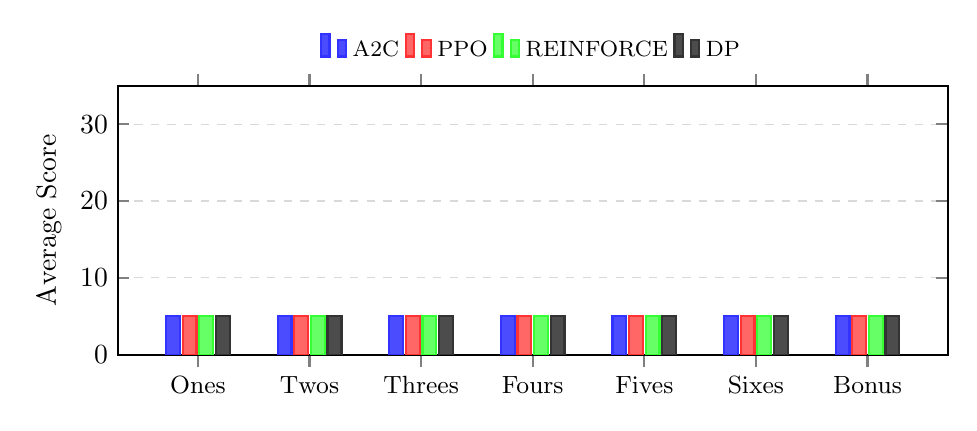
\begin{tikzpicture}
        \begin{axis}[
                ybar=1pt,
                width=\columnwidth,
                height=5cm,
                bar width=5pt,
                symbolic x coords={Ones,Twos,Threes,Fours,Fives,Sixes,Bonus},
                xtick=data,
                xticklabel style={font=\small},
                ylabel={Average Score},
                ymin=0,
                ymax=35,
                ymajorgrids=true,
                grid style={dashed,gray!30},
                legend style={
                        at={(0.5,1.05)},
                        anchor=south,
                        legend columns=4,
                        font=\footnotesize,
                        draw=none,
                        fill=none
                    },
                enlarge x limits=0.12,
                axis line style={thick},
                tick style={thick},
            ]

            % A2C
            \addplot[fill=blue!70!white, draw=blue!80!white, thick] coordinates {
                    (Ones,   5) (Twos,   5) (Threes, 5) (Fours,  5)
                    (Fives,  5) (Sixes,  5) (Bonus,  5)
                };

            % PPO
            \addplot[fill=red!60!white, draw=red!80!white, thick] coordinates {
                    (Ones,   5) (Twos,   5) (Threes, 5) (Fours,  5)
                    (Fives,  5) (Sixes,  5) (Bonus,  5)
                };

            % REINFORCE
            \addplot[fill=green!60!white, draw=green!80!white, thick] coordinates {
                    (Ones,   5) (Twos,   5) (Threes, 5) (Fours,  5)
                    (Fives,  5) (Sixes,  5) (Bonus,  5)
                };

            % DP
            \addplot[fill=black!70, draw=black!80, thick] coordinates {
                    (Ones,   5) (Twos,   5) (Threes, 5) (Fours,  5)
                    (Fives,  5) (Sixes,  5) (Bonus,  5)
                };

            \legend{A2C,PPO,REINFORCE,DP}

        \end{axis}
    \end{tikzpicture}
    \caption{Upper section and bonus scores (placeholder data)}
    \label{fig:category-upper}
\end{figure}


\begin{figure}[htb]
    \centering
    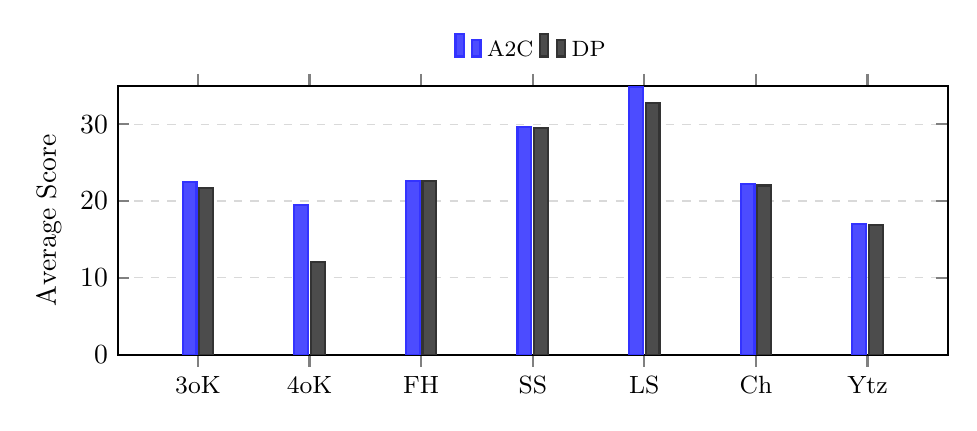
\begin{tikzpicture}
        \begin{axis}[
                ybar=1pt,
                width=\columnwidth,
                height=5cm,
                bar width=5pt,
                symbolic x coords={3oK,4oK,FH,SS,LS,Ch,Ytz},
                xtick=data,
                xticklabel style={font=\small},
                ylabel={Average Score},
                ymin=0,
                ymax=35,
                ymajorgrids=true,
                grid style={dashed,gray!30},
                legend style={
                        at={(0.5,1.05)},
                        anchor=south,
                        legend columns=4,
                        font=\footnotesize,
                        draw=none,
                        fill=none
                    },
                enlarge x limits=0.12,
                axis line style={thick},
                tick style={thick},
            ]

            % A2C
            \addplot[fill=blue!70!white, draw=blue!80!white, thick] coordinates {
                    (3oK,  22.42) (4oK,  19.47) (FH,   22.57) (SS,   29.63)
                    (LS,   34.80) (Ch,   22.22) (Ytz,  17.03)
                };


            % PPO
            %\addplot[fill=red!60!white, draw=red!80!white, thick] coordinates {
            %        (3oK,  5) (4oK,  5) (FH,   5) (SS,   5)
            %        (LS,   5) (Ch,   5) (Ytz,  5)
            %    };

            % REINFORCE
            %\addplot[fill=green!60!white, draw=green!80!white, thick] coordinates {
            %        (3oK,  5) (4oK,  5) (FH,   5) (SS,   5)
            %        (LS,   5) (Ch,   5) (Ytz,  5)
            %    };

            % DP
            \addplot[fill=black!70, draw=black!80, thick] coordinates {
                    (3oK,  21.66) (4oK,  12.10) (FH,   22.59) (SS,   29.46)
                    (LS,   32.71) (Ch,   22.01) (Ytz,  16.87)
                };

            \legend{A2C,DP}

        \end{axis}
    \end{tikzpicture}
    \caption{Lower section scores (placeholder data)}
    \label{fig:category-lower}
\end{figure}


\subsubsection{Strategy Comparison Across Agents}
We also compared some high-level strategy metrics across our different agents to understand how their learned policies differed.
First, we analyzed the distribution of the first category choice made by each agent in Figure \ref{fig:strategy-first-category}.
Next, we analyzed each category to understand at what point in the game the agent typically filled it, shown in Figure \ref{fig:strategy-fill-turn}.

\begin{figure}[htb]
    \centering
    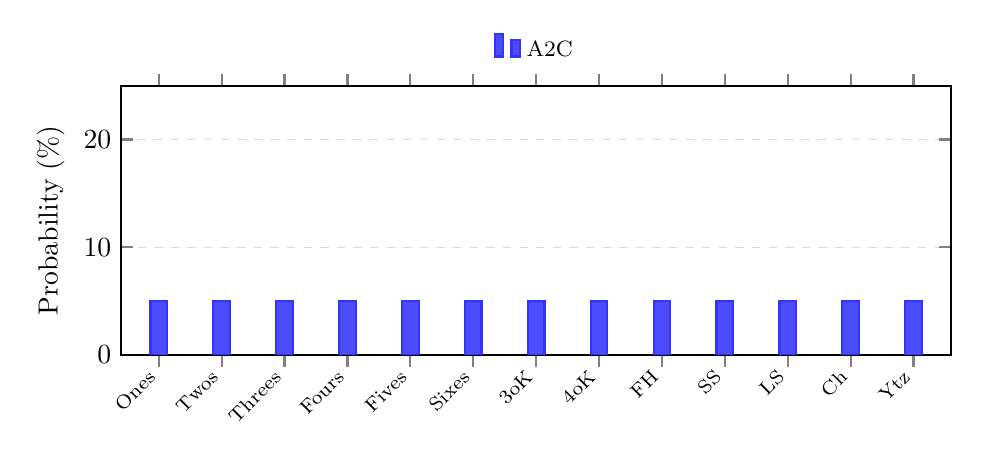
\begin{tikzpicture}
        \begin{axis}[
                ybar=1pt,
                width=\columnwidth,
                height=5cm,
                bar width=6pt,
                symbolic x coords={Ones,Twos,Threes,Fours,Fives,Sixes,3oK,4oK,FH,SS,LS,Ch,Ytz},
                xtick=data,
                xticklabel style={font=\scriptsize, rotate=45, anchor=east},
                ylabel={Probability (\%)},
                ymin=0,
                ymax=25,
                ymajorgrids=true,
                grid style={dashed,gray!30},
                legend style={
                        at={(0.5,1.05)},
                        anchor=south,
                        legend columns=3,
                        font=\footnotesize,
                        draw=none,
                        fill=none
                    },
                enlarge x limits=0.05,
                axis line style={thick},
                tick style={thick},
            ]

            % DP
            % \addplot[fill=black!70, draw=black!80, thick] coordinates {
            %         (Ones,5) (Twos,5) (Threes,5) (Fours,5) (Fives,5) (Sixes,5)
            %         (3oK,5) (4oK,5) (FH,5) (SS,5) (LS,5) (Ch,5) (Ytz,5)
            %     };

            % A2C
            \addplot[fill=blue!70!white, draw=blue!80!white, thick] coordinates {
                    (Ones,5) (Twos,5) (Threes,5) (Fours,5) (Fives,5) (Sixes,5)
                    (3oK,5) (4oK,5) (FH,5) (SS,5) (LS,5) (Ch,5) (Ytz,5)
                };

            % PPO
            % \addplot[fill=red!60!white, draw=red!80!white, thick] coordinates {
            %         (Ones,5) (Twos,5) (Threes,5) (Fours,5) (Fives,5) (Sixes,5)
            %         (3oK,5) (4oK,5) (FH,5) (SS,5) (LS,5) (Ch,5) (Ytz,5)
            %     };

            \legend{A2C}

        \end{axis}
    \end{tikzpicture}
    \caption{First category chosen distribution (placeholder data)}
    \label{fig:strategy-first-category}
\end{figure}


% \begin{figure}[H]
%     \centering
%     \begin{tikzpicture}
%         \begin{axis}[
%                 ybar=1pt,
%                 width=\columnwidth,
%                 height=5cm,
%                 bar width=8pt,
%                 symbolic x coords={Ones,Sixes,4oK,Ch,Ytz},
%                 xtick=data,
%                 xticklabel style={font=\small},
%                 ylabel={Median Fill Turn},
%                 ymin=0,
%                 ymax=13,
%                 ymajorgrids=true,
%                 grid style={dashed,gray!30},
%                 legend style={
%                         at={(0.5,1.05)},
%                         anchor=south,
%                         legend columns=3,
%                         font=\footnotesize,
%                         draw=none,
%                         fill=none
%                     },
%                 enlarge x limits=0.15,
%                 axis line style={thick},
%                 tick style={thick},
%             ]

%             % A2C
%             \addplot[fill=blue!70!white, draw=blue!80!white, thick] coordinates {
%                     (Ones,5) (Sixes,5) (4oK,5) (Ch,5) (Ytz,5)
%                 };

%             % PPO
%             \addplot[fill=red!60!white, draw=red!80!white, thick] coordinates {
%                     (Ones,5) (Sixes,5) (4oK,5) (Ch,5) (Ytz,5)
%                 };

%             \legend{A2C,PPO}

%         \end{axis}
%     \end{tikzpicture}
%     \caption{Median fill turn for key categories (placeholder data)}
%     \label{fig:strategy-fill-turn}
% \end{figure}




\section{Discussion}
% <400-600 words>

\subsection{Is there a tradeoff between single-turn and full-game performance?}
Our results seem to show that there indeed is a tradeoff between the single-game and full-game objectives.
The single turn agent achieved high scores, often higher than the full-game REINFORCE agent,
but failed to learn a coherent bonus strategy, as expected.

At lower performance levels, there is a strong correlation between single-turn and full-game performance, as shown in Figure~\ref{fig:single-vs-full-game},
but as full-game performance improves, the correlation weakens. We were also able to use significantly smaller models for the single-turn agent,
indicating that the full-game task is inherently more complex.
However, it would be interesting to see if transfer learning from single-turn to full-game agents could help improve sample efficiency.

\subsection{Can an agent reach optimal play?}
Our best full-game agent, trained with A2C, was able to reach a median score of 241.78 points over 100,000 evaluation games,
which is within 5.0\% of the optimal DP score of 254.59.
This indicates that with appropriate algorithm and architectural choices, it is indeed possible to approach near-optimal performance using self-play alone.

\subsection{Which design choices most affect final performance?}
Our ablation studies highlighted several design choices that significantly impacted final performance.
First, the choice of RL algorithm and credit assignment was crucial; A2C with TD(0) outperformed both PPO and REINFORCE in terms of stability and final score.
Second, the state and action encodings played a significant role; specifically providing (rather than forcing the network to learn) some easily calculable features improved learning.
Third, entropy regularization played a huge role in stabilizing training and encouraging exploration. This made the most difference in the model's intra-turn strategy.
Lastly, reward shaping was critical to learning the upper section bonus strategy, agents learned it extremely slowly without it.

\subsection{What failure modes exist in learned policies?}
Despite the strong performance of the Actor-Critic agent, we observed several failure modes in the learned policies.
Most notably, the agent still overweighted the four-of-a-kind category, even when pursuing the upper section bonus would have been more beneficial.
Likewise, the agent did not make good use of the Chance category, using it right off the bat rather than saving it for difficult endgame scenarios.
These failures highlight persistent long-horizon credit-assignment and exploration challenges, despite the use of reward shaping and entropy regularization.

\subsection{Further Improvements}
Our final training runs used a fixed budget of 1 million games. This took nearly 10 hours to train on a single NVIDIA A100 GPU.
Samples were often the bottleneck for learning, in fact the bonus performance had not fully converged even after this many games.
Further improvements to parallelization and GPU utilization could help reduce training time, allowing for larger budgets to be explored.
Likewise, we struggled to get larger batch sizes to work, this would likely improve training times as well.

A few other improvements could likely help close the gap further. For example, different types of learning rate schedules could be used.
Soft-Actor-Critic (SAC) \cite{haarnoja2018softactorcriticoffpolicymaximum} style entropy control could be used to more finely adapt exploration during training,
we had to tune entropy coefficients manually for each algorithm, and they often required large adjustments when other hyperparameters changed.


\section{Conclusion and Future Work}
% <200-300 words>

Learning a robust policy for \textit{Yahtzee} using reinforcement learning presents several interesting challenges and insights.
We showed that with appropriate algorithmic choices, it is possible to approach near-optimal performance using self-play alone.
Our results back up theoretical results in the literature regarding training stability and sample efficiency of common RL algorithms.
Our analysis of learned policies showed that these algorithms often struggle to learn rare, yet high-reward strategies, especially if they require strong coherence over longer time horizons.

Future research could be done to find architectures, samples, and learning methods that allow the model to better approximate optimal play, more efficiently.
Transfer learning could be explored further to see if knowledge from single-turn optimization could be effectively transferred to full-game, multiplayer Yahtzee, or other variants of the game.
For example, curriculum learning approaches, where the agent is gradually exposed to more complex scenarios over time, could be used to help the model overcome some challenges outlined in this paper.
For the multiplayer setting, future work could explore permutation-invariant architectures such as Deep Sets \cite{zaheer2018deepsets} or embeddings with self-attention to handle unsorted dice or opponent states\cite{vaswani-2017-attention}.
Additionally, \textrm{Yahtzee} could also be considered as a candidate environment for research into hierarchical reinforcement learning methods \cite{Barto2003}.


\bibliographystyle{acl_natbib}
\bibliography{csml_bibliography}

\clearpage
\appendix

\section{Reproducibility}
The code for this project is \href{https://github.com/papetronics/case-studies-final-project}{available on GitHub}.

Likewise, data for all experiments used in this graph is available in \href{https://wandb.ai/papetronics/yahtzee-final-project}{the Weights \& Biases report}.

The trained A2C full-game model can be found on \href{https://huggingface.co/papetronics/yahtzee-a2c-full-game}{HuggingFace}.

\section{Hyperparameters}
The following hyperparameters were used for the baseline models:

\begin{table}[H]
    \centering
    \small
    \caption{Shared hyperparameters across all algorithms}
    \label{tab:shared-hyperparameters}
    \begin{tabular}{lc}
        \hline
        \textbf{Hyperparameter}       & \textbf{Value} \\
        \hline
        $d_h$ (Hidden Size)           & 600            \\
        $L$ (Hidden Layers)           & 3              \\
        $p_d$ (Dropout Rate)          & 0.1            \\
        $r_{\alpha}$ (Min LR Ratio)   & 0.01           \\
        $B$ (Games per Batch)         & 20             \\
        Activation Function           & Swish          \\
        Rolling Action Representation & Categorical    \\
        \hline
    \end{tabular}
\end{table}

\begin{table}[H]
    \centering
    \small
    \setlength{\tabcolsep}{4pt}
    \caption{Algorithm-specific hyperparameters}
    \label{tab:algorithm-hyperparameters}
    \begin{tabular}{lccc}
        \hline
        \textbf{Hyperparameter}        & \textbf{REINFORCE} & \textbf{A2C} & \textbf{PPO} \\
        \hline
        $\alpha$                       & 0.001              & 0.0001       & 0.0001       \\
        $\gamma$ (min)                 & 0.95               & 0.99         & 0.99         \\
        $\gamma$ (max)                 & 1.0                & 0.99         & 0.99         \\
        $\tau_{\mathrm{clip}}$         & 0.0                & 1.0          & 1.0          \\
        $\lambda_V$                    & 0.025              & 0.005        & 0.01         \\
        $\beta_{\mathrm{roll}}$ (max)  & 0.1                & 0.06         & 0.02         \\
        $\beta_{\mathrm{roll}}$ (min)  & 0.01               & 0.02         & 0.005        \\
        $\beta_{\mathrm{score}}$ (max) & 0.02               & 0.03         & 0.05         \\
        $\beta_{\mathrm{score}}$ (min) & 0.003              & 0.008        & 0.01         \\
        Entropy Hold Period            & 0.1                & 0.3          & 0.1          \\
        Entropy Anneal Period          & 0.55               & 0.6          & 0.8          \\
        \hline
    \end{tabular}
\end{table}

\begin{table}[H]
    \centering
    \small
    \caption{PPO-specific hyperparameters}
    \label{tab:ppo-hyperparameters}
    \begin{tabular}{lc}
        \hline
        \textbf{Hyperparameter} & \textbf{Value} \\
        \hline
        PPO Clip $\epsilon$     & 0.2            \\
        PPO Games per Minibatch & 4              \\
        PPO Epochs              & 3              \\
        \hline
    \end{tabular}
\end{table}

\section{Compute Costs}
Experiments were collected using a mix of a local RTX 3090 and AWS-hosted Tesla T4 GPUs.
The total cost of cloud compute was approximately \textbf{\$130}.
Over \textbf{312} training runs were logged in Weights \& Biases, totaling approximately \textbf{566.59 GPU hours}.

\section{AI Usage}

This paper utilized artificial intelligence tools in the following ways:
\begin{itemize}
    \item \textbf{GitHub Copilot (Claude Sonnet 4.5)} was used for typesetting assistance with LaTeX/KaTeX, IDE autocomplete suggestions during coding, and to occassionally perform straightforward refactorings, CUDA performance optimizations, and debugging.
    \item \textbf{ChatGPT (GPT-5.1)} was used for brainstorming ideas for reinforcement learning applications in games, guidance in hyperparameter tuning, helping to outline the structure of this paper, assistance in discovering relevant research and citations, and for writing tone and quality feedback.
\end{itemize}
All other content, including research methodology, analysis, results interpretation, and conclusions, represents original work by the author. The AI tools were not used to generate substantive content or analysis in this document.

\section{Yahtzee Scoring Rules}
\label{app:scoring}
Next we define the indicator functions for each of the scoring categories:

\begin{align*}
    \mathbb{I}_{3\mathrm{k}}(\mathbf{d})
     & = \mathbb{I}\bigl\{ \max_{v} n_v(\mathbf{d}) \ge 3 \bigr\} \\
    \mathbb{I}_{4\mathrm{k}}(\mathbf{d})
     & = \mathbb{I}\bigl\{ \max_{v} n_v(\mathbf{d}) \ge 4 \bigr\} \\
    \mathbb{I}_{\mathrm{full}}(\mathbf{d})
     & = \mathbb{I}\Bigl\{
    \exists i, j \in \{1, \mathellipsis, 6 \} \ \text{with} \ n_i(\mathbf{d}) = 3 \land n_j(\mathbf{d}) = 2
    \Bigr\}                                                       \\
    \mathbb{I}_{\mathrm{ss}}(\mathbf{d})
     & = \mathbb{I}\Bigl\{
    \exists k \in \{1,2,3\} \ \text{with}\
    \sum_{v=k}^{k+3} \mathbb{I}\{n_v(\mathbf{d}) > 0\} = 4
    \Bigr\}                                                       \\
    \mathbb{I}_{\mathrm{ls}}(\mathbf{d})
     & = \mathbb{I}\Bigl\{
    \exists k \in \{1,2\} \ \text{with}\
    \sum_{v=k}^{k+4} \mathbb{I}\{n_v(\mathbf{d}) > 0\} = 5
    \Bigr\}                                                       \\
    \mathbb{I}_{\mathrm{yahtzee}}(\mathbf{d})
     & = \mathbb{I}\bigl\{\max_v n_v(\mathbf{d}) = 5\bigr\}
\end{align*}

The potential score for each category can then be defined as:
\begin{align*}
    f_j(\mathbf{d})        & = j \cdot n_j(\mathbf{d}), \qquad j \in \{1,\dots,6\}                   \\
    f_7(\mathbf{d})        & = \mathbf{1}^\top \mathbf{d} \cdot \mathbb{I}_{3\mathrm{k}}(\mathbf{d}) \\
    f_8(\mathbf{d})        & = \mathbf{1}^\top \mathbf{d} \cdot \mathbb{I}_{4\mathrm{k}}(\mathbf{d}) \\
    f_9(\mathbf{d})        & = 25 \cdot \mathbb{I}_{\mathrm{full}}(\mathbf{d})                       \\
    f_{10}(\mathbf{d})     & = 30 \cdot \mathbb{I}_{\mathrm{ss}}(\mathbf{d})                         \\
    f_{11}(\mathbf{d})     & = 40 \cdot \mathbb{I}_{\mathrm{ls}}(\mathbf{d})                         \\
    f_{12}(\mathbf{d})     & = 50 \cdot \mathbb{I}_{\mathrm{yahtzee}}(\mathbf{d})                    \\
    f_{13}(\mathbf{d})     & = \mathbf{1}^\top \cdot \mathbf{d}                                      \\
    \mathbf{f}(\mathbf{d}) & =
    \bigl(f_1(\mathbf{d}), f_2(\mathbf{d}), \ldots, f_{13}(\mathbf{d})\bigr)
\end{align*}

\section{State Transition Function}
\label{app:transition-function}

$P$ can be defined by the following generative process.

\begin{itemize}
    \item If $r < 2$ and $a = k$, for each die $i$:
          \begin{itemize}
              \item if $k_i = 1$, keep $d'_i = d_i$;
              \item else sample $d'_i \sim \mathrm{Unif}\{1,\dots,6\}$ independently.
          \end{itemize}
          Set $c' = c,\ r' = r+1,\ t' = t$.
    \item If $r = 2$ and $a = i$, set $d' = d$, update $c' = \mathrm{score}(c,d,i)$,
          set $r' = 0,\ t' = t+1$.
\end{itemize}

\end{document}
